%% LyX 2.2.3 created this file.  For more info, see http://www.lyx.org/.
%% Do not edit unless you really know what you are doing.
\documentclass[aps,prd,superscriptaddress,nofootinbib,showpacs,showkeys,floatfix]{revtex4}
\usepackage[latin9]{inputenc}
\setcounter{secnumdepth}{3}
\usepackage{xcolor}
\usepackage{amsmath}
\usepackage{amssymb}
\usepackage{graphicx}
\usepackage[unicode=true,
 bookmarks=false,
 breaklinks=false,pdfborder={0 0 1},backref=section,colorlinks=false]
 {hyperref}

\makeatletter

%%%%%%%%%%%%%%%%%%%%%%%%%%%%%% LyX specific LaTeX commands.
%% Because html converters don't know tabularnewline
\providecommand{\tabularnewline}{\\}

%%%%%%%%%%%%%%%%%%%%%%%%%%%%%% Textclass specific LaTeX commands.
\@ifundefined{textcolor}{}
{%
 \definecolor{BLACK}{gray}{0}
 \definecolor{WHITE}{gray}{1}
 \definecolor{RED}{rgb}{1,0,0}
 \definecolor{GREEN}{rgb}{0,1,0}
 \definecolor{BLUE}{rgb}{0,0,1}
 \definecolor{CYAN}{cmyk}{1,0,0,0}
 \definecolor{MAGENTA}{cmyk}{0,1,0,0}
 \definecolor{YELLOW}{cmyk}{0,0,1,0}
}

%%%%%%%%%%%%%%%%%%%%%%%%%%%%%% User specified LaTeX commands.
\PassOptionsToPackage{english}{babel}

\usepackage{float}
\usepackage{mathrsfs}
\usepackage{amsfonts}
\usepackage{array}
\usepackage{epsfig}
% need for subequations
% defines \lesssim, etc
% need for figures
% useful for program listings
% use if color is used in text
%\linespread{1.5}

\renewcommand{\thefootnote}{\fnsymbol{footnote}}
\def\ltap{\raisebox{-.6ex}{\rlap{$\,\sim\,$}} \raisebox{.4ex}{$\,<\,$}}
\def\gtap{\raisebox{-.6ex}{\rlap{$\,\sim\,$}} \raisebox{.4ex}{$\,>\,$}}
\def\lra{\leftrightarrow}
\def\naive{na\"{\i}ve}
\newcommand{\as}{\alpha_{\mathrm{S}}}
\newcommand{\f}[2]{\frac{#1}{#2}}
\def\beq{\begin{equation}}
\def\b0{\beta_0}
\def\bone{\beta_1}
\def\btwo{\beta_2}
\def\eeq{\end{equation}}
\def\beeq{\begin{eqnarray}}
\def\eeeq{\end{eqnarray}}
\def\bom#1{{\mbox{\boldmath $#1$}}}
\def\to{\rightarrow}
\def\ito{\leftarrow}
\def\nn{\nonumber}
\def\arrowlimit#1{\mathrel{\mathop{\longrightarrow}\limits_{#1}}}
\def\qt{q_T}
\newcommand{\asFPi}{\frac{\as}{4\pi}}
\def\ptmin{p_{T{\rm min}}}
\def\ptmax{p_{T{\rm max}}}
\def\ms{${\overline {\rm MS}}$}
\def\tL{{\widetilde L}}
\newcommand{\ib}{\bar{\imath}}

\makeatother

\begin{document}

\preprint{SMU-HEP-?-?}

\title{PDFsense Tasks and Results}

\author{Bo Ting Wang}

\affiliation{Department of Physics, Southern Methodist University,\\
 Dallas, TX 75275-0181, U.S.A. }

\author{Pavel~M. Nadolsky}

\affiliation{Department of Physics, Southern Methodist University,\\
 Dallas, TX 75275-0181, U.S.A. }
\begin{abstract}
{[}{*} UPDATE THE ABSTRACT {*}{]} % We demonstrate a collection of tools and metrics for quantitatively
% studying the sensitivity of hadronic measurements to the underlying
% Parton Distribution Functions (PDFs). \\
 \\
 \textcolor{red}{Replace PACS with PhySH:}\texttt{\textcolor{red}{https://www.aps.org/publications/apsnews/201602/classification.cfm}} 
\end{abstract}

\pacs{\textcolor{red}{12.15.Ji, 12.38 Cy, 13.85.Qk}}

\keywords{parton distribution functions; Large Hadron Collider; Higgs boson}

\maketitle
\newpage{}\tableofcontents{}\newpage{} % - - - - - - SECTION I - - - - - - - - - - - - - - - - - - - - - - -

\section{Introduction \label{sec:Introduction}}

......

\section{PDF preliminaries \label{sec:PDF-preliminaries}}

\subsection{Data residuals in a global QCD analysis \label{sec:Data-residuals}}

In the CTEQ-TEA global analysis, the $\chi^{2}$ function accounts
for multiple sources of experimental uncertainties, as well as for
some prior theoretical constraints on the $a_{l}$ parameters. Consequently,
the global $\chi^{2}$ function takes the form 
\begin{equation}
\text{\ensuremath{\chi}}_{global}^{2}=\sum_{E}\chi_{E}^{2}+\chi_{th}^{2},\label{chi2global}
\end{equation}
where the sum runs over all experimental data sets $(E);$ and $\chi_{th}^{2}$
imposes theoretical constraints. The complete formulas for $\chi_{E}^{2}$
and $\chi_{th}^{2}$ can be found in Ref.~\cite{Gao:2013xoa}. For
the purposes of this paper, we express $\chi_{E}^{2}$ for each experiment
$E$ in a compact form as a sum of squared\emph{ shifted residuals}
$r_{i}^{2}(\vec{a})$, which are summed over $N_{pts}$ individual
data points $i$ in this experiment: 
\begin{align}
\chi_{E}^{2}(\vec{a}) & =\sum_{i=1}^{N_{pts}}\,r_{i}^{2}(\vec{a}).\label{eq:chi2}
\end{align}
In turn, $r_{i}(\vec{a})$ for the $i^{th}$ data point is constructed
from the theoretical prediction $T_{i}(\vec{a})$ evaluated in terms
of PDFs, total uncorrelated uncertainty $s_{i}$, and the shifted
central data value $D_{i,sh}(\vec{a})$:
\begin{align}
r_{i}(\vec{a}) & =\frac{1}{s_{i}}\,\big(T_{i}(\vec{a})-D_{i,sh}(\vec{a})\big)\ .\label{eq:residual}
\end{align}

This representation arises because, due to the presence of correlated
systematic errors in many experimental data sets, $\chi_{E}^{2}$
is dependent on $N_{\lambda}$ nuisance parameters $\lambda_{\alpha}$
associated with the correlated systematic factors, in addition to
the PDF parameters $\vec{a}$ and theoretical parameters such as $\alpha_{s}(M_{Z})$
and particle masses. The $\lambda_{\alpha}$ parameters are optimized
for each $\vec{a}$ according to the analytic solution derived in
Appendix B of Ref.~\cite{Pumplin:2002vw}. Optimization effectively
shifts the central value $D_{i}$ of the data point by an amount determined
by the optimal nuisance parameters $\overline{\lambda}_{\alpha}(\vec{a})$
and the correlated systematic errors $\beta_{i\alpha}:$
\begin{equation}
D_{i}\rightarrow D_{i,sh}(\vec{a})=D_{i}-\sum_{\alpha=1}^{N_{\lambda}}\beta_{i\alpha}\overline{\lambda}_{\alpha}(\vec{a}).
\end{equation}
 

We point out that some alternative representations for $\chi^{2}$
include the correlated systematic errors via a covariance matrix $\left(\mbox{cov}\right)_{ij}$,
rather than the above mentioned CTEQ-preferred form that explicitly
operates with $\lambda_{\alpha}$. Various $\chi^{2}$ definitions
in use are reviewed in \cite{Ball:2012wy}, as well as in \cite{Alekhin:2014irh}.
On the other hand, the representations based operating with $\lambda_{\alpha}$
and $\left(\mbox{cov}\right)_{ij}$ are derivable from each other
\cite{Gao:2013xoa}. From an extension of the derivation in Ref.~\cite{Pumplin:2002vw},
we may relate the shifted residual to the covariance matrix at each
individual point as 
\begin{equation}
r_{i}(\vec{a})\ =\ s_{i}\sum_{j=1}^{N_{\mathit{pts}}}(\mathrm{cov}^{-1})_{ij}\,\left(T_{j}(\vec{a})-D_{j}\right),\label{eq:res-cov}
\end{equation}
where 
\begin{equation}
(\mathrm{cov}^{-1})_{ij}\ =\ \left[\frac{\delta_{ij}}{s_{i}^{2}}\,-\,\sum_{\alpha,\beta=1}^{N_{\lambda}}\frac{\beta_{i\alpha}}{s_{i}^{2}}A_{\alpha\beta}^{-1}\frac{\beta_{j\beta}}{s_{j}^{2}}\right]\ ,\label{eq:covmat}
\end{equation}
and 
\begin{equation}
A_{\alpha\beta}\ =\ \delta_{\alpha\beta}\,+\,\sum_{k=1}^{N_{\mathit{pts}}}\frac{\beta_{k\alpha}\beta_{k\beta}}{s_{k}^{2}}\ .
\end{equation}
Thus, even if the PDF analyses operates with the covariance matrix,
one is still able to determine the shifted residuals $r_{i}$ from
$\left(\mbox{cov}^{-1}\right)_{ij}$ using Eq.~(\ref{eq:res-cov}).
In this article, we conveniently follow the CTEQ methodology and obtain
$r_{i}(\vec{a})$ directly from the CTEQ-TEA fitting program, together
with optimal nuisance parameters $\overline{\lambda}_{\alpha}(\vec{a})$
and shifted central data values $D_{i,sh}(\vec{a}).$


\section{Quantifying distributions of residuals\label{sec:QuantifyingDistributionsOfResiduals}}

We have demonstrated that the multi-dimensional distribution of the
shifted residuals $r_{i}$ evaluated with Hessian eigenvector PDFs
reflects PDF dependence of individual data points. In this section,
we will focus on numerical metrics to assess the emerging geometrical
picture and to visualize the regions of partonic momentum fractions
$x$ and QCD factorization scales $\mu$ where the experiments impose
strong constraints on a given PDF-dependent observable $X$. 

\subsection{Correlations and sensitivities \label{sec:CorrelationsSensitivities}}

\subsubsection{Correlation cosine. }

The correlation, which we define following Refs.~\cite{Pumplin:2001ct,Nadolsky:2001yg,Nadolsky:2008zw,Gao:2017yyd}
according to 
\begin{equation}
C_{f}\,\equiv\,\mbox{Corr}[f,r_{i}]=\frac{\vec{\nabla f}\cdot\vec{\nabla r}_{i}}{\Delta f\,\Delta r_{i}},\label{eq:corr}
\end{equation}
encodes the quantitative relation between $f$ and $r_{i}$ and can
determine whether there \emph{can} exist a predictive relationship
between $f$ and goodness of fit to the $i$-th data point. The correlation
function $\mathrm{\mbox{Corr}}[X,Y]$ of the quantities $X,\,Y$ in
Eq.~(\ref{eq:corr}) represents the Hessian formalism realization
of the Pearson's correlation coefficient, which we express as 
\begin{align}
\mathrm{\mbox{Corr}}[X,Y] & =\frac{1}{4\Delta X\Delta Y}\sum_{j=1}^{N}(X_{j}^{+}-X_{j}^{-})(Y_{j}^{+}-Y_{j}^{-})\ ,\label{eq:corr-def}
\end{align}
the sum in these expressions being over the $j$ parameters of the
full PDF model space. 

\subsubsection{Sensitivity.}

We employ $\vec{\nabla f}\cdot\vec{\nabla r}_{i}$ again to define
the \textit{sensitivity} of the $i^{th}$ data point to $f$, 
\begin{equation}
S_{f}\equiv\frac{\vec{\nabla f}\cdot\vec{\nabla r}_{i}}{\Delta f\,\langle r_{0}\rangle_{E}}=\frac{\Delta r_{i}}{\langle r_{0}\rangle_{E}}\,C_{f}\ ,\label{eq:sens}
\end{equation}
where $\Delta r_{i}$ and $\langle r_{0}\rangle_{E}$ are computed
according to Eqs.~(\ref{DelX}) and (\ref{r0E}), respectively. In
other words, $\Delta r_{i}$ represents the variation of the residuals
across the set of Hessian error PDFs, which we normalize to the root-mean-squared
residual for a given experiment to reduce impact of random fluctuations
of the experimental data values $D_{i}$. 

Yet another possible definition, which we list for completeness, is
to normalize the sensitivity as 
\begin{equation}
S_{f}^{\prime}\equiv\frac{\vec{\nabla f}\cdot\vec{\nabla r}_{i}}{f_{0}\,\langle r_{0}\rangle_{E}}=\frac{\Delta f}{f_{0}}\,S_{f}\ .\label{eq:sens-prime}
\end{equation}
For instance, if $f$ is the PDF $f(x_{i},\mu_{i})$ at the same points
$\{x_{i},\mu_{i}\}$ as the data, the definition (\ref{eq:sens-prime})
de-emphasizes $S_{f}^{\prime}$ at those data points where the PDF
uncertainty$\Delta f(x_{i},\mu_{i})$ is small compared to the best-fit
PDF value $f_{0}(x_{i},\mu_{i})$. 


\section{Ranking tables for experiments}

We calculate the average and total sensitity for each experimental
data and apply the tables to rank the impact to PDFs for experiments.
We also classify experiments to various types to see impact to PDFs
for these types. Tables are in Appendix \ref{sec:Tables}. 

\clearpage\newpage

\section{Case study: various Processes in CTEQ-TEA Data \label{sec:CaseCTEQ-TEA}}

In the following sections, we show some interesting results of PDFsense
and some issues we can study further. We use following symbols at
the beginning of each issue and result to indicate the attributions
of them: \textbf{\textcolor{blue}{Y}}/\textbf{\textcolor{blue}{N}}
for completeness/non-completeness of issues and results. If issues
are not completed yet (\textbf{\textcolor{blue}{N}}), we provide other
attribution for them: \textbf{\textcolor{teal}{1}}/\textbf{\textcolor{teal}{2}}/\textbf{\textcolor{teal}{3}}
means the time we expect to take for this issue is short/median/long.
\textbf{\textcolor{red}{!}}/\textbf{\textcolor{red}{!!}}/\textbf{\textcolor{red}{!!!}}
means the importance for this issue is low/median/high.

\subsection{All processes in CT14 HERA2 + LHC new data}

...
\begin{enumerate}
\item {[}\textbf{\textcolor{blue}{Y}}{]} showing all experiments at (x,Q)
space of PDFs \ref{fig:all_expt_xQ_data}
\item {[}\textbf{\textcolor{blue}{Y}}{]} shows correlation, sensitivity,
and respective histograms \ref{fig:CorrSensH14}, \ref{fig:Corrgluon},
\ref{fig:Sensgluon}
\item {[}\textbf{\textcolor{blue}{Y}}{]} sensitivity to Higgs cross section
at 14 TeV indicate the PDF sensitive to the future LHC Higgs survey
\ref{fig:CorrSensH14} 
\item {[}\textbf{\textcolor{blue}{Y}}{]} sensitivity to gluon PDF shows
demonstrate that the constraint of gluon at small x region ($10^{-3}-10^{-5}$)
is from HERA2 data and LHC jet data provides a fluent constraint to
gluon at $x>10^{-3}$ \ref{fig:Corrgluon}, \ref{fig:Sensgluon}
\end{enumerate}
\begin{figure*}
\includegraphics[width=1\textwidth]{plots/processes/all_expt/Allexpt_xQbyexpt_xQ}
\caption{A graphical representation in $\{x,\mu\}$ space of the full data
set treated in the present analysis, designated as ``CTEQ-TEA''.
It corresponds to an expansion of the CT14HERA2 data \cite{Hou:2016nqm}
fitted in the most recent CT14 framework \cite{Dulat:2015mca}, including
measurements from Run II of HERA \cite{Abramowicz:2015mha}. }
\label{fig:all_expt_xQ_data} 
\end{figure*}

\begin{figure*}
\includegraphics[width=0.3\textwidth]{plots/processes/all_expt/Allexpt_corr_xQ+1_f8_samept}\ \ \
\includegraphics[width=0.3\textwidth]{plots/processes/all_expt/Allexpt_corrdr_xQ+1_f8_samept}
\caption{For the full CTEQ-TEA dataset of Fig.~\ref{fig:all_expt_xQ_data},
we show the absolute correlation $|C_{f}|$ and sensitivity $|S_{f}|$
associated with the 14 TeV Higgs production cross section $\sigma_{H^{0}}(14\,\mathrm{TeV})$.
Points with significant magnitudes of $|C_{f}|$ and $|S_{f}|$ are
highlighted with color. When only the $|C_{f}|$ plot at left is considered,
it is primarily a subpopulation of jet production data (diagonal open
and closed inverted triangles with $\mu\gtrsim100$ GeV) that exhibits
significant correlations, as well as some HERA DIS and $t\bar{t}$
production data points. Our novel definition for the sensitivity in
the right panel, on the other hand, reveals many more points that
have comparable potency for constraining the Higgs cross section.
In this case, the great bulk of the jet production points, including
many of the highest scale measurements, is important, as well as a
number of other processes at smaller $\mu$, such as DIS data from
HERA (Exp. ID 160), NMC (104) and CDHSW (108), Drell-Yan information
from E866 (204), $t\bar{t}$ (565-568) and high-$p_{T}$ $Z$ production,
and even some points obtained from $Z$ production at LHCb (246).
\label{fig:CorrSensH14}}
\end{figure*}

\begin{figure*}
\includegraphics[width=0.3\textwidth]{plots/processes/all_expt/corr_xQ+1_f0_samept_nohigh}\ \ \
\includegraphics[width=0.27\textwidth]{plots/processes/all_expt/Allexpt_corr_hist+1_f0_samept}
\caption{Two representations of the correlation $|C_{g}|(x_{i},\mu_{i})$ of
the gluon PDF $g(x,\mu)$ with the point-wise residual $r_{i}$ of
the augmented CT14HERA2 analysis; in the left panel we plot a histogram
showing the distribution of correlations over 5227 $\{x,\mu\}$ points.
In the right panel we show the $\{x_{i},\mu_{i}\}$ map of these correlations
for the full dataset. \label{fig:Corrgluon}}
\end{figure*}

\begin{figure*}
\includegraphics[width=0.3\textwidth]{plots/processes/all_expt/corrdr_xQ+1_f0_samept_nohigh}\ \ \
\includegraphics[width=0.27\textwidth]{plots/processes/all_expt/Allexpt_corrdr_hist+1_f0_samept}
\caption{Like Fig.\ref{fig:Corrgluon}, but for the gluon sensitivity $|S_{g}|(x_{i},\mu_{i})$
as defined in Eq.\textasciitilde{}(\textbackslash{}ref\{eq:sens\}).
\label{fig:Sensgluon}}
\end{figure*}

\subsection{DIS NC processes}
\begin{enumerate}
\item {[}\textbf{\textcolor{blue}{Y}}{]} flavours with the most sensitivity:
dbar, u, d, uval, dbar/udar, d/u. By Table \ref{tab7}, \ref{tab8}
\end{enumerate}

\subsection{DIS CC processes}
\begin{enumerate}
\item {[}\textbf{\textcolor{blue}{Y}}{]} flavours with the most sensitivity:
dbar, u, d, uval, dval. By Table \ref{tab7}, \ref{tab8}
\end{enumerate}

\subsection{HERA Run 2 (ID = 160)}
\begin{enumerate}
\item {[}\textbf{\textcolor{blue}{Y}}{]} flavours with the most sensitivity:
ubar, g, u. By Table \ref{tab7}, \ref{tab8}
\end{enumerate}

\subsection{Jet, $t\overline{t}$ and Zpt Processes}

......
\begin{enumerate}
\item {[}\textbf{\textcolor{blue}{Y}}{]} flavours with the most sensitivity,
jet datasets: g, H7, H8, H14. Zpt datasets: g, s, H14. ttbar datasets:
g, H7, H8. By Table \ref{tab7}, \ref{tab8}
\item {[}\textbf{\textcolor{blue}{Y}}{]} jet CMS and ATLAS data provide
the most fluent sensitivity to gluon, b, c, and Higgs processes \ref{fig:jet_ttbar_Zpt_new}.
\textcolor{red}{note: we will redo the uncertainties of CMS and ATLAS
dataset, so we need to update this result with the new .dta data.} 
\item {[}\textbf{\textcolor{blue}{Y}}{]} Although ttbar and Zpt are also
averagely sensitive to these flavours, they are not necessary when
we incorporate LHC jet data sets \ref{fig:jet_ttbar_Zpt_new}. 
\end{enumerate}
\begin{figure*}
 \ \ \
\includegraphics[clip,width=0.3\textwidth]{plots/processes/jet/new/corrdr_xQ+1_f8_samept} 

\includegraphics[clip,width=0.3\textwidth]{plots/processes/ttbar/corrdr_xQ+1_f8_samept}
\ \ \
\includegraphics[clip,width=0.3\textwidth]{plots/processes/Zpt/corrdr_xQ+1_f8_samept} 

\caption{up is LHC jet (542, 544, 545). left-down is ttbar (565\textasciitilde{}568).
right-down is Zpt (247, 253, 254, 255) events.}
\label{fig:jet_ttbar_Zpt_new}
\end{figure*}

\subsection{$W$ processes}
\begin{enumerate}
\item {[}\textbf{\textcolor{blue}{Y}}{]} flavours with the most sensitivity:
dbar, d, dval, dbar/ubar, d/u. By Table \ref{tab7}, \ref{tab8}
\item {[}\textbf{\textcolor{blue}{Y}}{]} new data (249) impose d, dbar,
d/u, dbar/ubar constraints \ref{fig:W_new}
\end{enumerate}
\begin{figure*}
\ \ \
\includegraphics[clip,width=0.3\textwidth]{plots/processes/W/new/corrdr_xQ+1_f13_samept} 

\caption{LHC W asymmetry data (249) }
\label{fig:W_new}
\end{figure*}

\subsection{$Z$ processes}
\begin{enumerate}
\item {[}\textbf{\textcolor{blue}{Y}}{]} flavours with the most sensitivity,
old Z datasets: dbar, ubar, u, dval, uval, dbar/ubar. new Z datasets:
dbar, ubar, u, s, d/u. By Table \ref{tab7}, \ref{tab8}
\end{enumerate}

\subsection{$W/Z$ processes}
\begin{enumerate}
\item {[}\textbf{\textcolor{blue}{Y}}{]} flavours with the most sensitivity,
old W/Z datasets: dbar, ubar, u, d, s, uval, dbar/ubar, d/u. new W/Z
datasets: dbar/ubar, d/u. By Table \ref{tab7}, \ref{tab8}
\end{enumerate}

\section{Case Study: LHeC and EIC \label{sec:Case-Study:-LHeC}}

......Here provide the prediction of the sensitivity analysis of LHeC\&JlabEIC
DIS NC and CC datasets \ref{tab:LHeC}. \textcolor{red}{} We analyze
the sensitivity with pseudodata provided by them and normalize the
sensitivity contribution to 1 year runtime and 10 years runtime to
indicate the future impact. The way we normalize is as follows: the
statistical uncertainties $\sigma_{uncor}\propto1/\sqrt{luminosity}\propto1/\sqrt{runtime}\propto1/r\propto1/\delta r$,
so the sensitivity is roughly proportional to $\sqrt{runtime}$. For
the given $n_{1}$ years pseudodata, we can always estimate the sensitivity
of $n_{2}$ years $S_{n2}$ is equal to $\sqrt{n_{2}/n_{1}}S_{n1}$.
Here we only consider the sensitivity from statistical errors so the
real impact on PDFs could be further reduced by the systematic error.
Here I show the sensitivity based on the 1-year runtime analysis. 

The whole sensitivity of colliders estimated as 10-year runtime is
$\sqrt{10}=3.16$ times more than the 1-year runtime sensitivity.
However, with the various ways to combine rawdata into bins, we can
get different number of bins and PDF sensitivities on bins. We perhaps
need to weigh the impact on PDFs of various experimental runtime/\#bins. 
\begin{enumerate}
\item {[}\textbf{\textcolor{blue}{Y}}{]} According to the 1-year ranking
table, LHeC CC $e^{-}p$ and EIC CC measurements (191\&196) contribute
much less sensitivities than other channels (\textasciitilde{}30\%
and \textasciitilde{}4\%).
\item {[}\textbf{\textcolor{blue}{Y}}{]} the large $\delta r$ enhance the
sensitivities of LHeC\&EIC data to PDFs especially at the large and
small x regions ($x>0.5\&x<10^{-3}$) \ref{fig:LHeCEIC1y-dr}
\item {[}\textbf{\textcolor{blue}{Y}}{]} LHeC DISNC datasets constrain the
small x ($x<10^{-3}$) region of the gluon PDF \ref{fig:LHeCEIC1y-sens},
\ref{fig:LHeCEIC1y-corr}
\item {[}\textbf{\textcolor{blue}{Y}}{]} LHeC\&EIC DISCC and DISNC datasets
constrain u and d at large x and small x regions ($x>0.5\&x<10^{-3}$).
For the small x region, the high sensitivity perhaps results from
few present constraints on PDFs in that region 
\item {[}\textbf{\textcolor{blue}{N}}\textbf{\textcolor{teal}{?}}\textbf{\textcolor{red}{!}}{]}
LHeC DISCC data is correlated to middle x region ($10^{-3}\sim10^{-2}$)
strange PDF, I don't know why \ref{fig:LHeCEIC1y-corr}. Perhaps the
strong correlation is due to the large uncertainty of the strange
PDF, which means some DISCC data could constrain strange at this region. 
\item {[}\textbf{\textcolor{blue}{N}}\textbf{\textcolor{teal}{?}}\textbf{\textcolor{red}{!}}{]}
I don't know why the diagonal part of 192, 194 (LHeC $e^{+}p$ NC
\& CC) points in Fig. \ref{fig:LHeCEIC1y-corr} are strongly correlated
with the ubar and dbar PDFs 
\item {[}\textbf{\textcolor{blue}{Y}}{]} we also want to draw the sensitivity
plots for the EIC at various energies and luminosities, using the
same setting as for the LHeCs. With the .dta files, we can generate
them instantly. 
\item {[}\textbf{\textcolor{blue}{N}}\textbf{\textcolor{teal}{3}}\textbf{\textcolor{red}{?}}{]}
Make the ranking tables for 1-year and 10-years runtime of LHeC and
JLabEIC. (update: I already made ranking tables, yet we need different
ways to present the contribution based on various runtime/\#bins)
\end{enumerate}
\begin{figure*}
\includegraphics[clip,width=0.3\textwidth]{plots/Pseudo_Data/LHeCEIC_1y/corrdr_xQ+1_f0_samept}
\ \ \
\includegraphics[clip,width=0.3\textwidth]{plots/Pseudo_Data/LHeCEIC_1y/corrdr_xQ+1_f2_samept} 

\caption{Select sensitivity plots for the LHeC\&EIC pseudodata, in this case
showing $|S_{g}|(x_{i},\mu_{i})$ in the left panel, $|S_{d}|(x_{i},\mu_{i})$
in the right. The pseudodata are broken among four separate reaction
channels for LHeC \textemdash{} CC $e^{-}p$ (circles) and $e^{+}p$
(squares), as well as NC $e^{-}p$ (diamonds) and $e^{+}p$ (triangles).
And two channels for EIC \textemdash{} NC (down-triangle) and CC (empty-circle).}
\label{fig:LHeCEIC1y-sens} 
\end{figure*}

\begin{figure*}

\includegraphics[clip,width=0.3\textwidth]{plots/Pseudo_Data/LHeCEIC_1y/corr_xQ+1_f3_samept}
\ \ \
\includegraphics[clip,width=0.3\textwidth]{plots/Pseudo_Data/LHeCEIC_1y/corr_xQ+1_f-1_samept} 

\caption{Select correlation plots for the LHeC\&EIC pseudodata, in this case
showing $|C_{s}|(x_{i},\mu_{i})$ in the left, and $|C_{\overline{u}}|(x_{i},\mu_{i})$
in the right. The pseudodata are broken among four separate reaction
channels for LHeC \textemdash{} CC $e^{-}p$ (circles) and $e^{+}p$
(squares), as well as NC $e^{-}p$ (diamonds) and $e^{+}p$ (triangles).
And two channels for EIC \textemdash{} NC (down-triangle) and CC (empty-circle).}
\label{fig:LHeCEIC1y-corr} 
\end{figure*}

\begin{figure*}
\includegraphics[clip,width=0.3\textwidth]{plots/Pseudo_Data/LHeCEIC_1y/dr_xQ+1_samept}

\caption{Select $\delta r$ plots for the LHeC\&EIC pseudodata, in this case
showing $\delta r_{i}$ in the left panel. The pseudodata are broken
among four separate reaction channels for LHeC \textemdash{} CC $e^{-}p$
(circles) and $e^{+}p$ (squares), as well as NC $e^{-}p$ (diamonds)
and $e^{+}p$ (triangles). And two channels for EIC \textemdash{}
NC (down-triangle) and CC (empty-circle).}
\label{fig:LHeCEIC1y-dr} 
\end{figure*}

......

\begin{table}[ht]
\begin{tabular}{|l|lr|c|c|c}
\hline 
\textbf{ID\#}  & \textbf{LHeC pseudodata set}  &  & $N_{pts}$  & Fig.~\ref{fig:LHeC} symbol  & lumi\tabularnewline
\hline 
\hline 
191  & LHeC CC $e^{-}p$  &  & 93  & circle  & $10fb^{-1}/1y;100fb^{-1}/10y$\tabularnewline
\hline 
192  & LHeC CC $e^{+}p$  &  & 109  & square  & $10fb^{-1}/1y;100fb^{-1}/10y$\tabularnewline
\hline 
193  & LHeC NC $e^{-}p$  &  & 128  & diamond  & $10fb^{-1}/1y;100fb^{-1}/10y$\tabularnewline
\hline 
194  & LHeC NC $e^{+}p$  &  & 148  & triangle  & $10fb^{-1}/1y;100fb^{-1}/10y$\tabularnewline
\hline 
195 & JLab EIC NC &  & 156 & down-triangle & $10fb^{-1}/1y;100fb^{-1}/10y$\tabularnewline
\hline 
196 & JLab EIC CC &  & 50 & empty-circle & $10fb^{-1}/1y;100fb^{-1}/10y$\tabularnewline
\hline 
\end{tabular}\caption{Separate channels of the unpolarized lepton-proton deep-inleastic
scattering pseudodata for the LHeC from Ref.~\cite{LHeCdata}. For
each channel, here we list the specific physical process, number of
associated pseudodata points, as well as the symbol indicating the
channel in the $|S_{f}|(x_{i},\mu_{i})$ plots of Fig.~\ref{fig:LHeC}. }
\label{tab:LHeC} 
\end{table}

\section{Case Study: Constraining Physical Qunatities}

\subsection{Some interesting Quantities}

If we can get the uncertainty replicas of following physical quantities,
we can use user function to draw the sensitivity plots instantly
\begin{enumerate}
\item {[}\textbf{\textcolor{blue}{Y}}{]} Higgs cross section at 7, 8, 14
TeV
\item {[}\textbf{\textcolor{blue}{N}}\textbf{\textcolor{teal}{?}}{]} Sensitivities
to the $W$ boson mass at ATLAS (Camarda)
\item {[}\textbf{\textcolor{blue}{N}}\textbf{\textcolor{teal}{?}}{]} weak
mixing angle at CMS (Arie Bodek)
\item {[}\textbf{\textcolor{blue}{N}}\textbf{\textcolor{teal}{?}}{]} constraints
on dim-6 operators (Alexey Petrov)
\item {[}\textbf{\textcolor{blue}{Y}}{]} sensitivities of correlated systematic
errors to various physical observables (Higgs cross sections, weak
angle, etc.)

In addition to uncorrelated errors, I also explore the sensitivities
to PDFs and physical quantities $Q$ imposed by correlated errors
of LHC measurements. For the i-th correlated error in the measurement
ID $\beta_{ID,i}$, we define it's sensitivities to PDFs and $Q$
as $S(\beta_{ID,i},f_{a}(x,\mu))=\delta\beta_{ID,i}C(\beta_{ID,i},f_{a}(x,\mu))$
and $S(\beta_{ID,i},Q)=\delta\beta_{ID,i}C(\beta_{ID,i},Q)$. Where
i denote the ordering of $\beta_{ID,i}$ in .dta files (labels ``r(k)
= $R^{2}$ $\beta_{ID,1}$ $\beta_{ID,2}$ $\beta_{ID,3}$......''
in .dta files)

I identify the $\beta_{ID,i}$ with strong enough sensitivities to
various PDFs and $Q$. Since $S(\beta_{ID,i},f_{a}(x,\mu))$ depend
on $x$ and $\mu$, I calculate the $S(\beta_{ID,i},f_{a}(x,\mu))$
at $\mu=5GeV$ and $x=10^{-5},10^{-4},10^{-3},10^{-2},10^{-1},0.3,0.8$
and use the maximum $|S(\beta_{ID,i},f_{a}(x,\mu))|$ among $x$ values
to stand for the sensitivity to the PDF of flavour $a$. Afterwards,
I list all $\beta_{ID,i}$ with $|S_{max}(\beta_{ID,i},f_{a}(x,\mu=5GeV))|>1$
and $|S(\beta_{ID,i},Q)|>1$ in (./Temporary\_Results/Constrain\_Physical\_Quantities\_tmp/Sens\_correlated\_error/MaxSenscorrerror\_info.txt
of https://smu.box.com/s/sdd9qbw6wvee6n7u6441j2f2jil7s2t7). Besides,
I illustrate the sensitivities with the green to red spectrum on the
$(\beta_{ID,i},ID)$ grid (Fig. \ref{fig:Sens_corr_error}). I find
that most $\beta_{ID,j}$ with large sensitivities are in ID = 247,
249, 542, 544, 545, 566, 568. Especially, $\beta_{ID,j}$ of 249 are
the most sensitive among all correlated errors; Almost all $|S|>3$
$\beta_{ID,j}$ are in 249 and the maximum is $|S_{max}(\beta_{249,7},f_{d}(10^{-4},5GeV))|=9.45$.

{[}\textbf{\textcolor{blue}{N}}\textbf{\textcolor{teal}{1}}\textbf{\textcolor{red}{!}}{]}
Compare $\underset{i}{\Sigma}|S(\beta_{ID,i},f_{a}(x,\mu))|$ with
$\underset{i}{\Sigma}|S(r_{ID,i},f_{a}(x,\mu))|$ for each ID and
flavour 
\begin{figure*}
\includegraphics[clip,width=0.3\textwidth]{plots/constrain_quantities/sens_correrror_+1_f8_thumbnail}

\caption{The $|S_{f}(\beta_{ID,j},\sigma_{H,8TeV})|$ for LHC datasets.}
\label{fig:Sens_corr_error} 
\end{figure*}
\item 
\end{enumerate}
\clearpage\newpage

\subsection{Estimate the Potential Gain }

{[}\textbf{\textcolor{blue}{N}}\textbf{\textcolor{teal}{3}}\textbf{\textcolor{red}{!!}}{]}
We can define $S'=(\delta Q/Q)S$ to de-emphasize the sensitivities
of physical quantities $Q$ with small uncertainty fractions. We assume
it is more beneficial to constrain physical quantities $Q$ with large
uncertainties.

\subsection{Mellin Moments }

......Compare with lattice predictions and constrain PDFs by applying
penalties to the PDFs that disagree with the lattice predictions in
the fit
\begin{enumerate}
\item {[}\textbf{\textcolor{blue}{Y}}{]} \ref{tab:Mellin_total_sens} provides
the Mellin moment quantities that accept the most sensitivities from
the HERA2 and LHC datasets, and the B-C and gluon PDFs are sensitive
to jet data \ref{fig:Mellin_B-C}
\item {[}\textbf{\textcolor{blue}{N}}\textbf{\textcolor{teal}{?}}\textbf{\textcolor{red}{!}}{]}
$(u^{-}-d^{-})x^{0}$ should be 1 (constant) but its total sensitivity
is the same amount compared with most Mellin moments (see row 1 and
2 in \ref{tab:Mellin_total_sens}). We can lower the order of precision
to reduce the fluctuations on it. However, it also indicates that
even physical quantities have no correlation/sensitivity with datasets/PDFs,
the numerical fluctuations still contribute some sensitivities to
PDFs. Therefore, to avoid considering the sensivities from fluctuations,
perhaps we don't want to consider too low sensitivity as the real
sensitivity. Perhaps we also want to figure out ways to remove the
fluctuations or identify whether the sources of sensitivities are
fluctuations.
\item {[}\textbf{\textcolor{blue}{N}}\textbf{\textcolor{teal}{1}}\textbf{\textcolor{red}{!!}}{]}
some Mellin moments are sensitive to data at a narrow x band such
as in Fig. \ref{fig:Melling_x-1x0}, \ref{fig:Mellin_x2x3}. This
perhaps indicates that Mellin moments can be well-measured by just
imposing strong constraints at specific regions of PDFs. One way to
clarify it is to draw $x^{n}f(x,\mu)_{a}$ as the function of x for
n = 1, 2, 3 and a = the flavour index. Assume that the peak of the
PDFs have the most strong sensitivity, the x bands in Fig. \ref{fig:Melling_x-1x0},
\ref{fig:Mellin_x2x3} should overlap with the peak of corresponding
$x^{n}f(x,\mu)_{a}$ at x-axis.
\item \textbf{({*} PN {*})} {[}\textbf{\textcolor{blue}{Y}}{]} The $\langle(1-x)^{N}\rangle_{F}$
moments may be sensitive to the small-$x$ behavior for the PDF combinations
that are integrable in the limit $x\rightarrow0$. A $\langle(1-x)^{N}\rangle_{F}$
is a linear combination of $\langle x^{k}\rangle_{F}$ moments: 
\begin{equation}
\langle(1-x)^{N}\rangle_{F}=\sum_{k=0}^{N}C_{k}^{N}\ (-1)^{k}\ \langle x^{k}\rangle_{F},
\end{equation}
where 
\begin{equation}
C_{k}^{N}\equiv\frac{N!}{k!(N-k)!}.
\end{equation}
Thus, $\langle(1-x)^{N}\rangle_{F}$ can be in principle derived from
the standard Mellin moments.

The non-singlet combinations $T_{3}^{\pm}$, $T_{8}^{\pm}$, $T_{15}^{\pm}$,
etc. are integrable at $x\rightarrow0$. For $T(x)=T_{3}^{+}(x)=u(x)+\overline{u}(x)-d(x)-\overline{d}(x)$,
we write 
\begin{eqnarray}
 & \langle1-x\rangle_{T}=\int_{0}^{1}dx\ \left(1-x\right)T(x)=\langle1\rangle_{T}-\langle x\rangle_{T};\\
 & \langle(1-x)^{2}\rangle_{T}=\langle1\rangle_{T}-2\langle x\rangle_{T}+\langle x^{2}\rangle_{T};\\
 & \langle(1-x)^{3}\rangle_{T}=\langle1\rangle_{T}-3\langle x\rangle_{T}+3\langle x^{2}\rangle_{T}-\langle x^{3}\rangle_{T}.
\end{eqnarray}
We can similarly compute $\langle(1-x)^{N}\rangle_{T}$ for $T(x)=T_{q}^{-}(x)=q(x)-\overline{q}(x)$
with $q=u,d,...$; as well as for $T(x)=T_{3}^{-}(x)=u(x)-\overline{u}(x)-d(x)+\overline{d}(x)$.
\end{enumerate}
Result: We make ranking tables and sensitivity plots for $x^{n}$,
$(1-x)^{n}$ (in PDFsense\_Tasks\_and\_Results of SMU box). For $(1-x)^{n}$,
the flavours that HERA2 points are sensitive to have the most total
sensitivity because of the large amount of HERA2 points (e.g. T24)
\ref{fig:Melling_1-xn}. Also, the sensitivities are not sensitive
to order $n$ and the high sensitive $x$ regions are in $(10^{-2},1)$,
which seems means that it is hard to measure the small $x$ PDFs through
Melling moments $(1-x)^{n}q(x)$. Besides, we find that W/Z datasets
and BCDMS, CDHSW, CCFR, NuTeV, HERA2 datasets contribute the most
total sensitivity to the flavours we investigate, indicating that
DIS and VBP events are main sources of the sensitivities to the Melling
moments. 

\textcolor{red}{note: the total sensitivity table uses the old formula,
it should be modify latter}

\begin{figure*}
\includegraphics[clip,width=0.3\textwidth]{plots/MellinMoment/corrdr_xQ+1_f55_samept}

\includegraphics[clip,width=0.3\textwidth]{plots/MellinMoment/corrdr_xQ+1_f57_samept}

\caption{data sets sensitivity to the 1st and 3rd order B-C of Melling moment}
\label{fig:Mellin_B-C} 
\end{figure*}

\begin{table}[ht]
\begin{tabular}{|l|lr}
\hline 
\textbf{ID\#}  & \textbf{\textbar{}S\textbar{}}  & \textbar{}S\textbar{} for the respective quantities\tabularnewline
\hline 
\hline 
most  & 350\textasciitilde{}450 & 500\textasciitilde{}1000\tabularnewline
\hline 
$(u^{-}-d^{-})x^{0}$ & 418. & 590.\tabularnewline
\hline 
B-C\textasciicircum{}2 & 788. & 928.\tabularnewline
\hline 
B-C\textasciicircum{}3 & 848. & 928.\tabularnewline
\hline 
T15\textasciicircum{}2 & 501. & 843.\tabularnewline
\hline 
T15\textasciicircum{}3 & 530. & 843.\tabularnewline
\hline 
T24\textasciicircum{}3 & 536. & 826.\tabularnewline
\hline 
g\textasciicircum{}2 & 794. & 907.\tabularnewline
\hline 
g\textasciicircum{}3 & 851. & 907.\tabularnewline
\hline 
\end{tabular}\caption{The sensitivity of mellin moments quantities and the respective non-mellin
moment quantities imposed by HERA2 + LHC datasets}
\label{tab:Mellin_total_sens} 
\end{table}

\begin{figure*}
\includegraphics[clip,width=0.3\textwidth]{plots/MellinMoment/x0x-1_corr/corr_xQ+1_f28_samept}

\caption{datasets correlation to $x^{-1}$ of Melling moment }
\label{fig:Melling_x-1x0} 
\end{figure*}

\begin{figure*}
\includegraphics[clip,width=0.3\textwidth]{plots/MellinMoment/x2x3_corr/corr_xQ+1_f18_samept}

\ \ \
\includegraphics[clip,width=0.3\textwidth]{plots/MellinMoment/x2x3_corr/corr_xQ+1_f22_samept} 

\caption{data sets sensitivity to $x^{2}$, $x^{3}$ of Melling moment}
\label{fig:Mellin_x2x3} 
\end{figure*}
\begin{figure*}
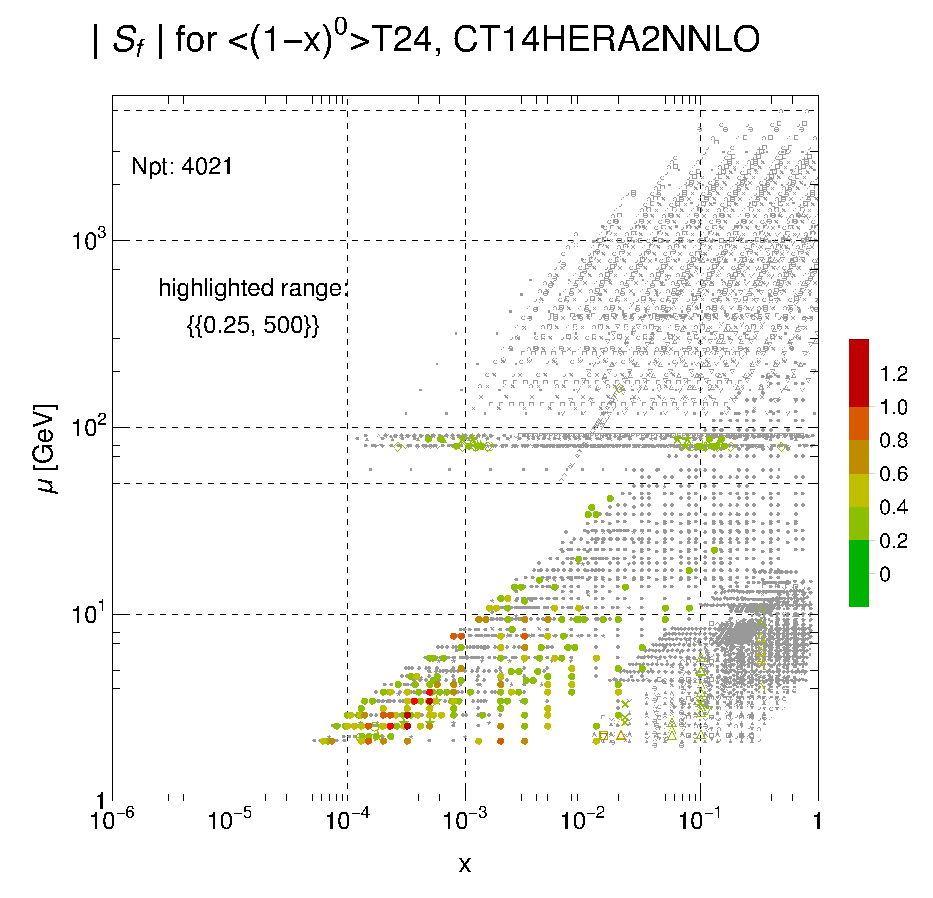
\includegraphics[clip,width=0.3\textwidth]{plots/MellinMoment/1-x/corrdr_xQ+1_f34_samept}

\caption{datasets correlation to $x^{-1}$ of Melling moment }
\label{fig:Melling_1-xn} 
\end{figure*}

\section{Case Study: comparison of the fit with jets and with no jets}

...the HERA2 and HERA2NoJet are PDFsets with old jet datasets (504,
514, 535, 538) and without jet datasets in the fits. Here we compare
the sensitivities to HERA2 and HERA2NoJet PDFs imposed by the HERA2
+LHC datasets.
\begin{enumerate}
\item {[}\textbf{\textcolor{blue}{Y}}{]} this comparison shows the possible
sensitivity impacts when incorporating data sets in the fit of PDFsets
\ref{tab:HERA2_HERA2NoJet_total_sens}, \ref{fig:HERA2_HERA2NoJet_r_dr},
\ref{fig:HERA2_HERA2NoJet_corr_sens}
\item {[}\textbf{\textcolor{blue}{Y}}{]} after incorporating jet datasets
into the fit, both the total correlation and $\delta r$ values decrease,
so the total sensitivity is weakened.
\item {[}\textbf{\textcolor{blue}{Y}}{]} the total sensitivity difference
for the HERA2 and HERA2NoJet are mostly from old and new jet data
(see row 1, 2, and 3 in \ref{tab:HERA2_HERA2NoJet_total_sens}), so
the old jet data in the fit actually mostly constrain the PDF space
associated with jet processes
\item {[}\textbf{\textcolor{blue}{Y}}{]} because the PDF space associated
with jet processes is close to the space of ttbar/Zpt processes, which
is mainly associated with the gluon PDF, ttbar and Zpt gluon are expected
to be constrained by old jet data. From tab. \ref{tab:HERA2_HERA2NoJet_total_sens},
we find that the $\delta r$ and sensitivity of HERA2 are smaller
than which of HERA2NoJet, verifying that the old jet datasets impose
a remarkable constraint to ttbar/Zpt processes.
\item {[}\textbf{\textcolor{blue}{N}}\textbf{\textcolor{teal}{2}}\textbf{\textcolor{red}{!!}}{]}
Via comparing the change of the sensitivities, correlations, and $\delta r$
in 504, 514, 535, 538, we can observe how well the sensitivity factor
predicts the impact of incorporating datasets into the global fit
to the constraint on PDFs. e.g. We can examine the relations between
$S(r_{i},f_{a}(x_{i},\mu_{i}))$ and $\delta r_{i,HERA2}/\delta r_{i,HERA2NoJet}$
or $\delta f_{a,HERA2}(x_{i},\mu_{i})/\delta f_{a,HERA2NoJet}(x_{i},\mu_{i})$
for points $i$ to see whether the sensitivities indicate the degree
of the gained constraint on PDFs .
\item {[}\textbf{\textcolor{blue}{Y}}{]} reciprocate distance formula: $rd_{i}=(Npt-N_{sameID}/Npt)*1/(\sum_{i_{ID}\text{\ensuremath{\neq}}j_{ID}}^{Npt}|\stackrel{\rightharpoonup}{v_{i}}-\stackrel{\rightharpoonup}{v_{j}}|)$,
where $\stackrel{\rightharpoonup}{v_{i}}$ is the vector of PCA-reduced
10 dimensions of the normalized residuals ($\stackrel{\rightharpoonup}{\delta r}/r_{ID,rms}$)
in the space spanned by the Hessian-uncertainties replicas. The comparison
of reciprocate distances for normalized residuals of datasets to HERA2
and HERA2NoJet PDFsets shows that 234, 266, 203 are in average more
far away to other data in the replica space of normalized residuals
\ref{fig:HERA2_HERA2NoJet_rd3}. In the LHC datasets, 245, 249, 250,
542, 545 perhaps discover more new PDF space than others. Besides,
the ordering of the average reciprocate distances in the bar chart
for two PDFsets are similar. So first, the structure of normalized
residuals for most experiments are not affected by old jet datasets.
Second, most points in HERA2NoJet datasets are not neighboring to
points in old and new (LHC) jet datasets in the PCA-reduced space.
Hence, the fits with old jet datasets do not constrain the similar
space of PDFs to most experiments in the fit of HERA2NoJet. 
\item {[}\textbf{\textcolor{blue}{N}}\textbf{\textcolor{teal}{1}}\textbf{\textcolor{red}{!!}}{]}
For the experiments with the most points that are far away from other
points at space, we find that 234, 203, 266, 160, 124, 542, 249 have
the comparable larger maximum distances. We find that many experiments
in this list have just little data points, so it indicates that the
number of points in datasets is not the only factor affecting the
number of points providing the unique PDF constraint. The reciprocate
distance distributions in various experiments are very different.
For answering the question about which experiments have more faraway
points, perhaps we need to also do some statistics for the points
larger than a cut (e.g. $rd_{i}>\mu_{rd}+\sigma_{rd}$ for $i$ represents
the index of data points in all experiments) 
\end{enumerate}
\textcolor{red}{note: 1. The title of HERA2NoJet figures \ref{fig:HERA2_HERA2NoJet_rd3}
are not correct, which is still ``CT14HERA2 NNLO''. 2. Because I
use the plotted data with multiple points specified by .dta points,
the distances estimation of VBP, Jet, ttbar data are not correct.
I should use the normalized residuals of .dta data to calculate the
reciprocate distance. }

\begin{table}[ht]
\begin{tabular}{|l||llrrrrrrrrrrr}
\hline 
\textbf{ID\#}  & Npt & \textbf{\textbar{}r\textbar{}yes}  & \textbf{\textbar{}r\textbar{}no}  & \textbf{\textbar{}dr\textbar{}yes}  & \textbf{\textbar{}dr\textbar{}no}  & \textbf{\textbar{}Cg\textbar{}yes}  & \textbf{\textbar{}Cg\textbar{}no}  & \textbf{\textbar{}Sg\textbar{}yes}  & \textbf{\textbar{}Sg\textbar{}no}  & \textbf{\textbar{}Cs\textbar{}yes}  & \textbf{\textbar{}Cs\textbar{}no}  & \textbf{\textbar{}Ss\textbar{}yes}  & \textbf{\textbar{}Ss\textbar{}no} \tabularnewline
\hline 
\hline 
All & 5227 & 4857. & 5345. & 3835. & 4979. & 1398. & 1636. & 847. & 1215. & 693. & 901. & 450. & 677.\tabularnewline
\hline 
jet old  & 666 & 478. & 554. & 266. & 537. & 242. & 298. & 106. & 224. & 79. & 140. & 33. & 103.\tabularnewline
\hline 
jet new & 804 & 860. & 1250. & 874. & 1707. & 390. & 420. & 337. & 522. & 135. & 195. & 117. & 230.\tabularnewline
\hline 
ttbar & 35 & 26. & 43. & 18. & 34. & 18. & 20. & 10. & 14. & 3.9 & 3.7 & 2.1 & 2.6\tabularnewline
\hline 
Zpt & 53 & 79. & 82. & 26. & 32. & 25. & 32. & 6.5 & 11.1 & 18. & 16. & 5.6 & 5.7\tabularnewline
\hline 
\end{tabular}\caption{Total sensitivities comparison of HERA2 and HERA2NoJet. jet old: 504,
514, 535, 538. All: HERA2 data + new data (LHC jet, ttbar, Zpt, W/Z).
jet new: 42, 544, 545. ttbar: 565, 566, 567, 568. Zpt: 247, 253, 254,
255 }
\label{tab:HERA2_HERA2NoJet_total_sens} 
\end{table}

\begin{figure*}
\includegraphics[clip,width=0.3\textwidth]{plots/HERA2_HERA2NoJet/HERA2/residual_xQ+1_samept_thumb}
\ \ \
\includegraphics[clip,width=0.3\textwidth]{plots/HERA2_HERA2NoJet/HERA2NoJet/residual_xQ+1_samept_thumb} 

\includegraphics[clip,width=0.3\textwidth]{plots/HERA2_HERA2NoJet/HERA2/dr_xQ+1_samept_thumb}
\ \ \
\includegraphics[clip,width=0.3\textwidth]{plots/HERA2_HERA2NoJet/HERA2NoJet/dr_xQ+1_samept_thumb} 

\caption{the $r$, $\delta r$ of HERA2 and HERA2NoJet datasets}
\label{fig:HERA2_HERA2NoJet_r_dr} 
\end{figure*}

\begin{figure*}
\includegraphics[clip,width=0.3\textwidth]{plots/HERA2_HERA2NoJet/HERA2/corr_xQ+1_f0_samept_thumb}
\ \ \
\includegraphics[clip,width=0.3\textwidth]{plots/HERA2_HERA2NoJet/HERA2NoJet/corr_xQ+1_f0_samept_thumb} 

\includegraphics[clip,width=0.3\textwidth]{plots/HERA2_HERA2NoJet/HERA2/corrdr_xQ+1_f0_samept_thumb}
\ \ \
\includegraphics[clip,width=0.3\textwidth]{plots/HERA2_HERA2NoJet/HERA2NoJet/corrdr_xQ+1_f0_samept_thumb} 

\caption{the correlation and sensitivity of datasets to HERA2 and HERA2NoJet }
\label{fig:HERA2_HERA2NoJet_corr_sens} 
\end{figure*}

\begin{figure*}
\includegraphics[clip,width=0.3\textwidth]{plots/HERA2_HERA2NoJet/rd3/CT14HERA2NNLOall_AbsSens_newSens_formula_cutbrokenpoints/residual_all_norm_Reciprocate_distance_rd3B}
\ \ \
\includegraphics[clip,width=0.3\textwidth]{plots/HERA2_HERA2NoJet/rd3/HERA2_no_jet/residual_all_norm_Reciprocate_distance_rd3B} 

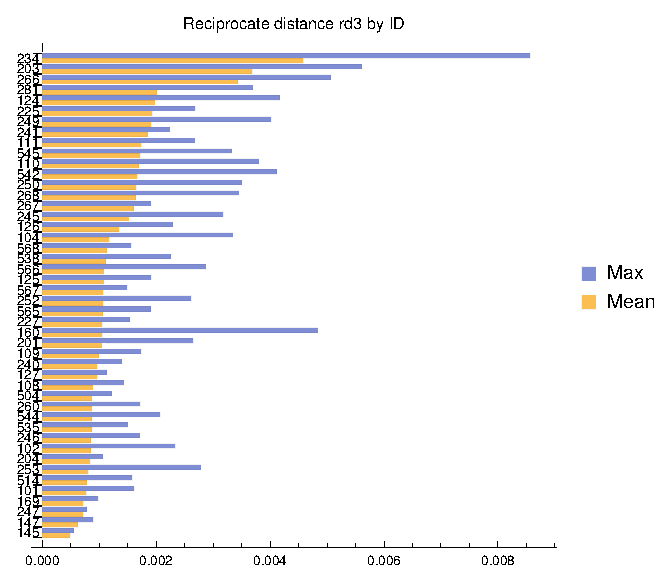
\includegraphics[clip,width=0.45\textwidth]{plots/HERA2_HERA2NoJet/rd3/CT14HERA2NNLOall_AbsSens_newSens_formula_cutbrokenpoints/residual_all_norm_Reciprocate_distance_ID_max_mean}
\ \ \
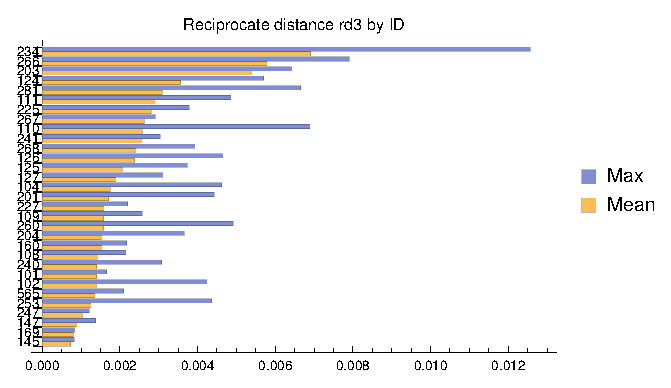
\includegraphics[clip,width=0.45\textwidth]{plots/HERA2_HERA2NoJet/rd3/HERA2_no_jet/residual_all_norm_Reciprocate_distance_ID_max_mean} 

\caption{the reciprocate distances among normalized residuals of points in
datasets. left-up: the HERA2 reciprocate distances. right-up: the
HERA2NoJet reciprocate distance. left-down: the mean and maximum of
the HERA2 reciprocate distances by experiments. right-down: the mean
and maximum of the HERA2NoJet reciprocate distances by experiments.}
\label{fig:HERA2_HERA2NoJet_rd3}
\end{figure*}

\section{Classifying Datasets}

This section we discuss methods of classifying datasets by the uncertainty
replicas of them. Via these methods, we could specify whether datasets
are correlated to the similar PDF region.
\begin{enumerate}
\item {[}\textbf{\textcolor{blue}{N}}\textbf{\textcolor{teal}{2}}\textbf{\textcolor{red}{!}}{]}
applying PCA and t-SNE algorithm to $\stackrel{\rightharpoonup}{\delta r}/r_{ID,rms}$,
we can efficiently separate it to different types, which means these
algorithms specify the diversity of the constraint imposed by datasets
\ref{fig:PCA_t-SNE}. We can compare the groups separated by t-SNE
to see what kind of datasets are relative to the similar PDFs, so
we can know a. whether incorporating a new dataset provides the constraint
we never have. b. the correlation relation between two processes (perhaps
even any nonlinear correlation relation could be explored).
\item {[}\textbf{\textcolor{blue}{N}}\textbf{\textcolor{teal}{3}}\textbf{\textcolor{red}{!!}}{]}
use the reciprocate distance to specify the uniqueness of datasets
perhaps is not the best way. We can use other quantities such as the
angles among points to define the similarity among points or use some
clustering algorithm to define jets in the replica space (or the space
of the PCA of the replicas).
\end{enumerate}
\begin{figure*}
\includegraphics[clip,width=0.3\textwidth]{plots/HERA2_HERA2NoJet/tensorprojector/pca}
\ \ \
\includegraphics[clip,width=0.3\textwidth]{plots/HERA2_HERA2NoJet/tensorprojector/tsne}

\caption{Distributions of displaced residuals $\vec{\delta_{i}}$ from the
CTEQ-TEA analysis obtained by dimensionality reduction methods. Left:
a 3-dimensional projection of a 10-dimensional manifold constructed
by principal component analysis (PCA). Right: a distribution from
the 3-dimensional t-SNE clustering method. Blue, orange, and red colors
indicate data points from DIS, vector boson production, and jet/$t\bar{t}$
production processes.}
\label{fig:PCA_t-SNE} 
\end{figure*}

\section{Other researches }

\subsection{Quantifying the sensitivity to PDFs in a x-range }

{[}\textbf{\textcolor{blue}{N}}\textbf{\textcolor{teal}{2}}\textbf{\textcolor{red}{!!!}}{]}
We try to quantify and visualize the constraint on a $x$ and $\mu$
range of PDFs imposed by experimental measurements. For the selected
data points or datasets, we can easily know the expected regions of
PDFs impacted by them. The total sensitivities to PDFs versus x at
$Q_{0}=1.3$ GeV is the most important result we want to see for this
idea. We can also use this tool to advanced study a. the total sensitivities
for each experimental ID and type of process. b. the comparison of
the constraint on PDFs for HERA2 and HERA2Nojet. 

The idea of quantifying the sensitivity to the whole x range of PDFs
imposed by experimental measurements is to draw the function $S(r_{i},f_{a}(x,\mu))$
in the x interval $[10^{-5},1]$ for each data point $i$ and flavour
$a$. We can know the sensitivity to the PDF of any flavour and any
(x,mu) range for the selected datasets by superposing the functions
$S(r_{i},f_{a}(x,\mu))$ of all points $i$. 

The finished part: a. The total sensitivities for the selected IDs,
showing all flavours in one plot (The left plot in Fig. \ref{fig:HERA2_sens_xrange}).
b. The total sensitivities for the selected IDs, showing the total
sensitivities of IDs separately (The right plot in Fig. \ref{fig:HERA2_sens_xrange}).
The left and middle plots in Fig. \ref{fig:HERA2_sens_xrange} implies
that HERA2 + LHC new datasets allocate the sensitivities evenly to
$10^{-5}<x<1$ and the total sensitivity to PDFs is not sensitive
to the factorization scale $\mu$. The right plot ranks the sensitivities
imposed by various datasets and demonstrates that 542 and 545 impose
the most sensitivities to the gluon PDF at large $x$ region. c. plot
the sensitivities at different $Q$: the left and middle plots show
that the total sensitivity to PDFs is not sensitive to the factorization
scale $Q$. d. generate the plot for each ID separately (in ./PDFsense\_Tasks\_and\_Results
of SMU box). \textcolor{red}{note: the 542 and 545 datasets need to
be replaced by the new version later (the right figure in \ref{fig:HERA2_sens_xrange}).}

{[}\textbf{\textcolor{blue}{N}}\textbf{\textcolor{teal}{2}}\textbf{\textcolor{red}{!!}}{]}
The functions we could add: a. The mean sensitivities. c. show the
total sensitivities for all IDs and the total sensitivities for each
ID in the same plot. 

\begin{figure*}
\includegraphics[clip,width=0.3\textwidth]{plots/sens_xrange/Sens_xrange_HERA2plusLHC_CT14HERA2NNLO_Q1_3}
\ \ \
\includegraphics[width=0.3\textwidth]{plots/sens_xrange/Sens_xrange_HERA2plusLHC_CT14HERA2NNLO_Q125}\ \ \
\includegraphics[clip,width=0.3\textwidth]{plots/sens_xrange/HERA2_LHC_JP_TTbar_Zpt_singlesens_g} 

\caption{Left: The total sensitivities to HERA2 PDFs in $10^{-5}<x<1$ at $Q=1.3$
GeV imposed by datasets in the HERA2 fit+LHC new datasets. Middle:
the same as the left figure yet $Q=125$ GeV. Right: The gluon sensitivities
for the LHC jet, ttbar, and ZpT datasets at $Q=1.3$ GeV.}
\label{fig:HERA2_sens_xrange} 
\end{figure*}

\subsection{construct theoretical predictions are the linear combination of different
flavour PDFs }

We want to know which direction in the PDF space (the PDF space means
the 6 dimensions spanned by $f_{\bar{d}}$ to $f_{s}$ at $(x,\mu)$
specified by data points) do datasets constrain rather than just know
the sensitivities of PDFs for various flavours. There are various
advandages. First, the constrained PDF direction and it's sensitivity
is more informative for identifying the constraint of datasets to
PDFs than sensitivities of PDFs for various flavours. Besides, We
don't need to guess and test which combination of flavour has the
strongest constraint by the user function again and again. We can
extract the information from the constrained direction. In addition,
if we know the relation between the theoretical values and PDFs, we
can possibly directly estimate the sizes of PDF uncertainties imposed
by datasets (seems the reweighting method could do the similar thing).
We can also investigate the distribution of the directions to illustrate
which directions are more correlated with various datasets and the
strength of sensitivities to these directions (which are roughly proportional
to residuals of data points).

We approximate that theoretical uncertainties are the linear combination
of PDF uncertainties at the specified $(x,\mu)$ plus an unknown term
$X$. That is: $(T_{i,r}-T_{i,0})=\underset{a}{\sum}c_{i,a}(f(x_{i},\mu_{i})_{a,r}-f(x_{i},\mu_{i})_{a,0})$
for $T$, $c$, and $f$ denote the theoretical values, linear coefficients,
and PDFs, $i$ denotes data points, $r$ denotes error replicas, and
0 denotes the central replica. Note: we do not use $T_{i,r}=\underset{a}{\sum}c_{i,a}f(x_{i},\mu_{i})_{a,r}+const$
as we can not get the well-fitted result. Here we temporary ignore
the nonlinear terms and the contribution from PDFs that are not at
$(x,\mu)$. We can do the linear regression between the error replicas
of theoretical predictions and PDFs to acquire the linear relation.
Because of replicas are far more than the 6 (the number of flavours
in the fit), the quality of the linear regression should be acceptable.
Following we derive the relation between theoretical/residual and
PDF uncertainties and connect to the concept of correlation/sensitivity
mentioned before: defining Hessian uncertainties of theoretical predictions
and PDFs:

\[
\delta T_{i,R}=(T_{i,r+}-T_{i,r-})/2,\delta f_{i,R}=(f_{i,r+}-f_{i,r-})/2
\]

\[
|\stackrel{\rightharpoonup}{\delta T_{i}}|^{2}=\stackrel[R]{N}{\sum}\delta T_{i,R}^{2},|\stackrel{\rightharpoonup}{\delta f_{i}}|^{2}=\stackrel[R]{N}{\sum}\delta f_{i,R}^{2}
\]

The linear relation between theoretical errors and PDF errors:

\[
(T_{i,r}-T_{i,0})=\underset{a}{\sum}c_{i,a}(f(x_{i},\mu_{i})_{a,r}-f(x_{i},\mu_{i})_{a,0})+(X_{i,r}-X_{i,0})
\]

\[
\delta T_{i,R}=\underset{a}{\sum}c_{i,a}(f_{i,a,r+}-f_{i,a,r-})/2+(X_{i,r+}-X_{i,r-})/2\equiv\underset{a}{\sum}c_{i,a}\delta f_{i,a,R}+\delta X_{i,R}
\]

Where $r+$, $r-$ denote the pairwisely positive and negative error
replicas in one of the total $N$ PDF model dimensions and $R$ denotes
the error in that dimension. $T$ are the theoretical predictions;
$f$ are PDFs; $i$ are data points; $a$ are flavour indices of $\overset{-}{d}$,
$\overset{-}{u}$,..., $s$. $c_{i,a}$ are the coefficients of the
$f_{i,a}$. $X$ are unknown parts. The symbols $\stackrel{\rightharpoonup}{\delta T_{i}}$,
$\stackrel{\rightharpoonup}{\delta f_{i}}$, and etc represent $N$
dimensional vectors with Hessian errors $\delta T_{i,R}$, $\delta f_{i,R}$,
and etc in each component so that $\stackrel{\rightharpoonup}{|\delta T_{i}}|$,
$\stackrel{\rightharpoonup}{|\delta f_{i}}|$, and etc are the Hessian
uncertainties of the given physical quantities $T_{i}$, $f_{i}$,
and etc. 

Because the total PDF uncertainties of physical quantities follow
the Hessian uncertainty rule: $|\stackrel{\rightharpoonup}{\delta Q}|=\sqrt{\stackrel[R]{N}{\sum}\delta Q_{R}^{2}}$
and the square of the addition of two vectors is $(\stackrel{\rightharpoonup}{Q_{1}}+\stackrel{\rightharpoonup}{Q_{2}})^{2}=|\stackrel{\rightharpoonup}{Q_{1}}|^{2}+|\stackrel{\rightharpoonup}{Q_{2}}|^{2}+2|\stackrel{\rightharpoonup}{Q_{1}}||\stackrel{\rightharpoonup}{Q_{2}}|\rho$
for the correlation $\rho$ between $\stackrel{\rightharpoonup}{Q_{1}}$
and $\stackrel{\rightharpoonup}{Q_{2}}$ , the total theoretical uncertainty
for each point $i$ is:

\[
|\stackrel{\rightharpoonup}{\delta T_{i}}|^{2}=\underset{R}{\sum}(\underset{a}{\sum}c_{i,a}\delta f_{i,a,R}+\delta X_{i,R})^{2}=|(\stackrel{\rightharpoonup}{\delta\underset{a}{\sum}c_{i,a}f_{i,a}})|^{2}+|\stackrel{\rightharpoonup}{\delta X_{i}}|^{2}+2|(\delta\stackrel{\rightharpoonup}{\underset{a}{\sum}c_{i,a}f_{i,a}})||\stackrel{\rightharpoonup}{\delta X_{i}}|\rho
\]

\[
\simeq|(\stackrel{\rightharpoonup}{\delta\underset{a}{\sum}c_{i,a}f_{i,a}})|^{2}+|\stackrel{\rightharpoonup}{\delta X_{i}}|^{2}
\]

Where we assume the unknown quantity $X$ and the known PDF combination
is uncorrelated ($\rho\simeq0$), which means that the vectors $\stackrel{\rightharpoonup}{\delta X_{i}}$,
$\stackrel{\rightharpoonup}{\delta\underset{a}{\sum}c_{i,a}\delta f_{i,a}}$
and $\stackrel{\rightharpoonup}{\delta T_{i}}$ form a right triangle.
Therefore, the Hessian uncertainty correlation between $\stackrel{\rightharpoonup}{\delta T_{i}}$
and $\stackrel{\rightharpoonup}{\underset{a}{\delta\sum}c_{i,a}f_{i,a}}$
is $C(T_{i},\underset{a}{\sum}c_{i,a}f_{i,a})=cos\theta_{\stackrel{\rightharpoonup}{\delta T_{i}},\stackrel{\rightharpoonup}{\underset{a}{\delta\sum}c_{i,a}f_{i,a}}}\simeq\frac{|\delta\stackrel{\rightharpoonup}{\underset{a}{\sum}c_{i,a}f_{i,a}}|}{|\stackrel{\rightharpoonup}{\delta T_{i}}|}$,
which indicates that $C(T_{i},\underset{a}{\sum}c_{i,a}f_{i,a})$
could be seen as the percentage of theoretical uncertainties explained
by $f_{\bar{d}}$,..., $f_{s}$. If even the various PDFs of flavours
are uncorrelated with each other, we have $C(T_{i},f_{i,a})\simeq\frac{(c_{i,a}|\stackrel{\rightharpoonup}{\delta f_{i,a}}|)}{|\stackrel{\rightharpoonup}{\delta T_{i}}|}$.
The physical explanation for the formulas is that the theoretical
uncertainty is the error propagation of linear independent uncertainties
of PDFs $f_{\bar{d}}$, $f_{\bar{u}}$, $f_{g}$, $f_{u}$, $f_{d}$,
$f_{s}$, and unknown $X$. Therefore, $c_{\bar{d}}(x,\mu),c_{\bar{u}}(x,\mu),c_{g}(x,\mu),c_{u}(x,\mu),c_{d}(x,\mu),c_{s}(x,\mu)$
specify the relation between uncertainties on PDFs of flavours and
experimental measurements.

\subsubsection{Setup}

for each dataset, using the linear fit $(T_{i,r}-T_{i,0})=\underset{a}{\sum}c_{i,a}(f(x_{i},\mu_{i})_{a,r}-f(x_{i},\mu_{i})_{a,0})$
to fit the 56 error replicas for each point $i$

\subsubsection{Verification of the linear independent approximation}

To know whether the linear approximation works well, here are some
ideas.
\begin{enumerate}
\item {[}\textbf{\textcolor{blue}{Y}}{]} by checking the relation $C(T_{i},\underset{a}{\sum}c_{i,a}f_{i,a})\simeq\frac{|\delta\stackrel{\rightharpoonup}{\underset{a}{\sum}c_{i,a}f_{i,a}}|}{|\stackrel{\rightharpoonup}{\delta T_{i}}|}$
in the left of Fig. \ref{fig:linearfitByPDFs_verify}, we verify the
formula. e.g. ID = 247 satisfies the relation and the goodness of
the specification (correlations) of points are very high.
\item {[}\textbf{\textcolor{blue}{N}}\textbf{\textcolor{teal}{2}}\textbf{\textcolor{red}{!}}{]}
by checking the p-values of coefficients $c_{i,a}$; there should
be at least one $a$ satisfying $p_{i,a}<0.05$ for each point $i$.
(X)
\item {[}\textbf{\textcolor{blue}{N}}\textbf{\textcolor{teal}{2}}\textbf{\textcolor{red}{!}}{]}
check the correlations of the linear fits are large enough for most
points (X)
\end{enumerate}

\subsubsection{physical problems and applications}

Note: results are in ./Temporary\_Results/other\_ideas\_tmp/LinearFitPDFs\_tmp/
of https://smu.box.com/s/sdd9qbw6wvee6n7u6441j2f2jil7s2t7

With $c_{\bar{d}}(x,\mu),c_{\bar{u}}(x,\mu),c_{g}(x,\mu),c_{u}(x,\mu),c_{d}(x,\mu),c_{s}(x,\mu)$,
we are able to study how measurements constrain PDFs. Here are some
problems we presently want to do: 
\begin{enumerate}
\item {[}\textbf{\textcolor{blue}{Y}}{]} make the statistical quantities
to represent the generic coefficients $c_{n}$ for each dataset (e.g.
the mean $<c_{n}>$ for flavours $n$): Because the points in each
datasets (even in the similar $x$ ranges) have very different coefficient
values or even ratios, taking the mean $<c_{n}>$is often not representative
for datasets. For example, the $c_{n}$ in datasets have large variance
and many outliers. Displaying the $c_{n}$ versus $(x,\mu)$ is perhaps
better. 
\item {[}\textbf{\textcolor{blue}{Y}}{]} visualization of the coefficients
of points for each experimental measurement on $(x,\mu)$ plane: We
make the coefficient fractions to the dominate coefficient. The way
to determine the dominant coefficient for each Expt ID is by ordering
the number of points of each flavour with the maximum $c_{n}$. The
flavour with the most number of points with maximum coefficients among
various flavours is used to normalize the coefficients for the corresponding
Expt ID. In the right Fig. \ref{fig:linearfitByPDFs_verify}, we find
that the $c_{\bar{d}}(x,\mu)-c_{\bar{u}}(x,\mu)$ is the largest coefficient
in ID = 203 and it becomes less dominant when $x>0.3$.
\item {[}\textbf{\textcolor{blue}{Y}}{]} quantify the strength of constraint
on the PDF space imposed by measurements and compare it with the components
from PDF uncertainties of flavours (which flavours contribute the
most to the theoretical uncertainties of measurements): Defining the
sensitivity $S(T_{i},\underset{a}{\sum}c_{i,a}f_{i,a})\equiv\frac{\delta r_{i}}{r_{ID,rms}}C(\delta r_{i},\underset{a}{\sum}c_{i,a}f_{i,a})\simeq\frac{|\delta\stackrel{\rightharpoonup}{\underset{a}{\sum}c_{i,a}f_{i,a}}|}{\sigma_{uncor,i}r_{ID,rms}}\simeq\frac{|\delta\stackrel{\rightharpoonup}{\underset{a}{\sum}c_{i,a}f_{i,a}}|}{\sigma_{uncor,i}}$,
we can investigate the $\underset{a}{\sum}c_{i,a}f_{i,a}$ sensitivities
on $(x,\mu)$ plane. To estimate the how much $f_{i,a}(x,\mu)$ contribute
to the $\underset{a}{\sum}c_{i,a}f_{i,a}$ sensitivities, we assume
the uncertainties of $c_{n}\delta f_{n}$ are independent, so $S(r_{i},\underset{a}{\sum}c_{i,a}f_{i,a})\simeq\frac{\sqrt{\underset{a}{\sum}(c_{i,a}|\delta f_{i,a}|/\sigma_{uncor,i})^{2}}}{r_{ID,rms}}$
indicates that the components of the best fit sensitivity $S(r_{i},\underset{a}{\sum}c_{i,a}f_{i,a})$
depends on sizes of of $c_{n}\delta f_{n}$. Here we provide an example
of ID = 203 sensitivity analysis for the best fit $\underset{a}{\sum}c_{i,a}f_{i,a}$,
where we hide the information of $\mu$ for the convinience and plot
$S(r_{i},\underset{a}{\sum}c_{i,a}f_{i,a})$ versus $x$ for each
Expt ID. From the middle of Fig. \ref{fig:linearfitByPDFs_verify}
we find that ID = 203 measures the $f_{d_{+}}-f_{u_{+}}$ and $S(T_{i},\underset{a}{\sum}c_{i,a}f_{i,a})$
decreases by $x$, which perhaps results from the decreasing of the
dominant coefficients $c_{\bar{d}}\delta f_{\bar{d}}$, $c_{\bar{u}}\delta f_{\bar{u}}$.
Even at the same $x$ value, $c_{n}\delta f_{n}$ could still be unstable,
which means that sometimes the coefficients $c_{n}$ somehow have
large uncertainties. In some measurements, the $c_{n}$ uncertainties
are very large (e.g. ID = 160). We also find that the approximation
$S(r_{i},\underset{a}{\sum}c_{i,a}f_{i,a})\simeq\frac{\sqrt{\underset{a}{\sum}(c_{i,a}|\delta f_{i,a}|/\sigma_{uncor,i})^{2}}}{r_{ID,rms}}$
is not always correct. For instance, part of the line of $c_{\bar{d}}\delta f_{\bar{d}}/\sigma_{uncor}$
is higher than $S(r_{i},\underset{a}{\sum}c_{i,a}f_{i,a})$ and $r_{ID,rms}\simeq1$,
contradicting to $S(r_{i},\underset{a}{\sum}c_{i,a}f_{i,a})\simeq\frac{\sqrt{\underset{a}{\sum}(c_{i,a}|\delta f_{i,a}|/\sigma_{uncor,i})^{2}}}{r_{ID,rms}}$. 
\item {[}\textbf{\textcolor{blue}{N}}\textbf{\textcolor{teal}{3}}\textbf{\textcolor{red}{?}}{]}
whether the sizes of components are representive for the sensitivities
of PDFs in the definition $S(T_{i},\underset{a}{\sum}c_{i,a}f_{i,a})\equiv\frac{\delta r_{i}}{r_{ID,rms}}C(\delta r_{i},\underset{a}{\sum}c_{i,a}f_{i,a})$.
In other words, in which conditions $\frac{|c_{i,a}(\delta f_{i,a})|}{\sigma_{uncor}}=\delta r_{i}C(r_{i},f_{i,a})$
\item {[}\textbf{\textcolor{blue}{N}}\textbf{\textcolor{teal}{?}}\textbf{\textcolor{red}{?}}{]}
can the knowledge of coefficients help us to rank the constraint on
PDFs imposed by measurements better?
\item {[}\textbf{\textcolor{blue}{N}}\textbf{\textcolor{teal}{3}}\textbf{\textcolor{red}{!!}}{]}
backward: how good the combination of measurements measure (reconstruct)
PDFs $f_{a}(x,\mu)$: $f_{a,R}(x,\mu)=\underset{R}{\sum}\delta T_{i,R}$
\item {[}\textbf{\textcolor{blue}{N}}\textbf{\textcolor{teal}{?}}\textbf{\textcolor{red}{?}}{]}
can the knowledge of coefficients help us to quantify the sensitivities
to physical quantities (e.g. $\sigma_{H}$)?
\item {[}\textbf{\textcolor{blue}{N}}\textbf{\textcolor{teal}{3}}\textbf{\textcolor{red}{!!!}}{]}
use this technique with HERA2/HERA2\_No\_Jet PDFsets to quantify the
potential $c_{i,n}\delta f_{i,n}/\sigma_{uncor,i}$ constraint on
ID = 504/514/535/538
\item {[}\textbf{\textcolor{blue}{N}}\textbf{\textcolor{teal}{1}}\textbf{\textcolor{red}{!!}}{]}
investigate the Q dependency of $S(r_{i},\underset{a}{\sum}c_{i,a}f_{i,a})$ 
\item {[}\textbf{\textcolor{blue}{N}}\textbf{\textcolor{teal}{3}}\textbf{\textcolor{red}{!!}}{]}
we can not fit the relation $T_{i,r}=\underset{a}{\sum}c_{i,a}f(x_{i},\mu_{i})_{a,r}+const$
well (the constant terms are oftenly too large and $C(T_{i},\underset{a}{\sum}c_{i,a}f_{i,a})\ncong\frac{|\stackrel{\rightharpoonup}{\underset{a}{\sum}c_{i,a}f_{i,a}}|}{|\stackrel{\rightharpoonup}{T_{i}}|}$
). If it is caused by the contribution of PDFs that are not at $(x,\mu)$,
the LO PDF should fit well. Test it with CT14LO.
\item {[}\textbf{\textcolor{blue}{N}}\textbf{\textcolor{teal}{3}}\textbf{\textcolor{red}{!}}{]}
Test the stability of coefficients of datasets. Coefficients in $(T_{i,r}-T_{i,0})=\underset{a}{\sum}c_{i,a}(f(x_{i},\mu_{i})_{a,r}-f(x_{i},\mu_{i})_{a,0})+(X_{i,r}-X_{i,0})$
relation should not depend on the datasets incorporated in PDF fits.
Via comparing the fitted coefficients in data points of CT14HERA2NNLO
and CT14HERA2NNLONoJet, we can verify it.
\end{enumerate}

\subsubsection{a temporary conclusion}
\begin{enumerate}
\item the statistical quantities (average, median, etc) is not a good way
to reveal the properties of coefficient $c_{n}$ for various flavours
$n$
\item $T_{i}=\underset{a}{\sum}c_{i,a}f_{i,a}+const$ does not satisfy $C(T_{i},\underset{a}{\sum}c_{i,a}f_{i,a})=\underset{a}{\sum}c_{i,a}f_{i,a}/T_{i}$.
I can not tell whether $T_{i}=\underset{a}{\sum}c_{i,a}f_{i,a}+const$
is a reasonable approximation. Instead, we can verify the approximation
$C(T_{i},\underset{a}{\sum}c_{i,a}f_{i,a})\simeq\frac{|\delta\stackrel{\rightharpoonup}{\underset{a}{\sum}c_{i,a}f_{i,a}}|}{|\stackrel{\rightharpoonup}{\delta T_{i}}|}$
is acceptable and provides some useful information about the PDF sensitivity
imposed by datasets. 
\item we display the $c_{n}$ versus $x$ to demonstrate the measured PDF
space depend on $x$ (assuming that the PDFs at different factorization
scale $\mu$ are strongly correlated and $f(x,\mu)\simeq f(x)$) 
\item $S(r_{i},\underset{a}{\sum}c_{i,a}f_{i,a})$ and $c_{i,n}\delta f_{i,n}/\sigma_{uncor,i}$
versus $x$ indicates the sensitivity depending on $x$ and the proportion
of the sensitivity components from various flavours $n$. However,
the correlations among different $\delta f_{i,n}$ are also important
and our analysis does not include the sensitivity contribution from
$C(f_{n1}(x,\mu),f_{n2}(x,\mu))$.
\item the $c_{n}$ in many datasets are numerical unstable or have large
uncertainties. When considering the $\mu$ dependency, we find that
$c_{n}$ strongly depend on $(x,\mu)$, so even $c_{n}$ and their
ratios spread widely even in same datasets.
\item large $c_{n}$ does not mean the $f_{n}$ is the main source of the
corresponding theoretical uncertainty or $f_{n}$ is the most sensitive
flavour. For instance, the $c_{\bar{u}}(x,\mu)$ of jet datasets are
mostly the largest among flavour coefficients but the $c_{g}\delta f_{g}$
is the largest among $c_{n}\delta f_{n}$. Perhaps it is the considerable
$\delta f_{g}$ that enhances the gluon sensitivities for jet and
ttbar datasets.
\item It seems that when the dominant $c_{n}\delta f_{n}$ are not far larger
than other $c_{n}\delta f_{n}$ , the correlations and sensitivities
would become lower.
\end{enumerate}
\begin{figure*}
\includegraphics[clip,width=0.3\textwidth]{plots/LinearFitPDFs/Corr_dfxQoverdTPearsonC_247}
\ \ \
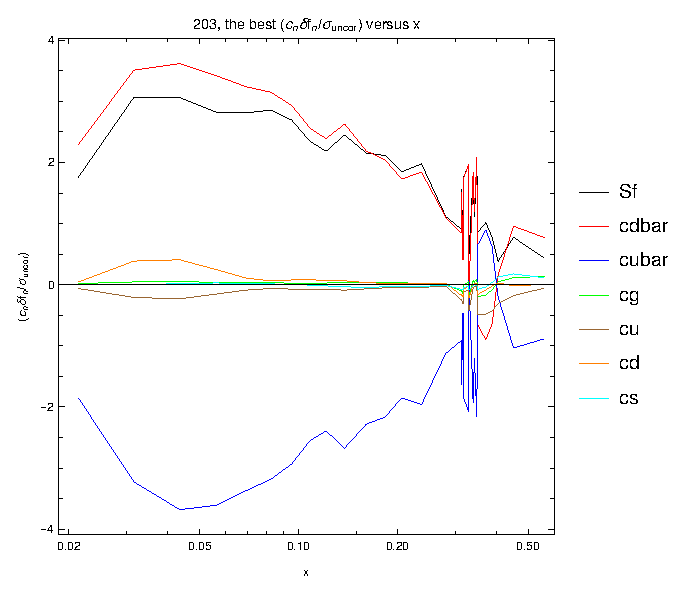
\includegraphics[clip,width=0.3\textwidth]{plots/LinearFitPDFs/BestFit_coefsdfNorm_vs_x_203}
\ \ \
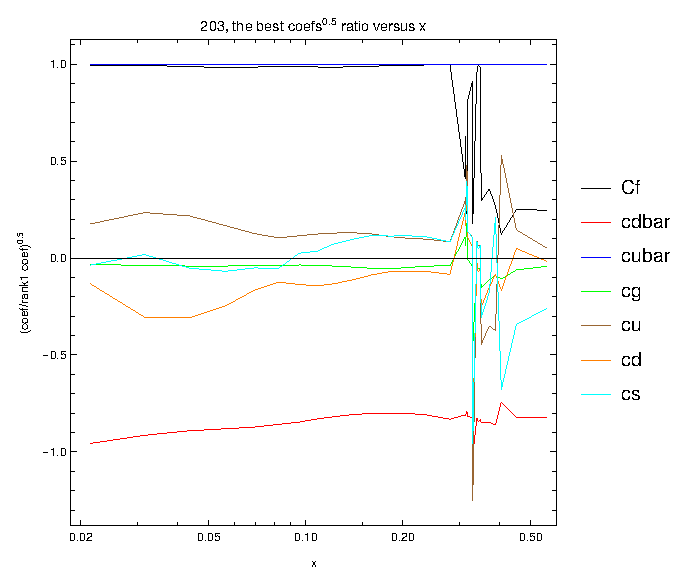
\includegraphics[clip,width=0.3\textwidth]{plots/LinearFitPDFs/BestFit_coefsRatio_vs_x_203}

\caption{left: The $C(T_{i},\protect\underset{a}{\sum}c_{i,a}f_{i,a})$ versus
$\frac{|\protect\underset{a}{\delta\sum}(c_{i,a}\delta f_{i,a})|}{|\delta T_{i}|}$
for ID = 247. middle: sensitivities of ID = 203 data depend on x.
right: coefficient fractions to the dominate coefficient depend on
x. }
\label{fig:linearfitByPDFs_verify} 
\end{figure*}

\section{Conclusions \label{sec:Conclusions}}

......

\subsection*{Acknowledgements}

......

\clearpage \newpage{}

\bibliographystyle{apsrev}
\bibliography{PDFsense_material}

\clearpage \newpage{}

\appendix

\section{Approximate kinematical variables\label{sec:supp}}

......

\section{Tabulated results \label{sec:Tables}}

......This Appendix we show the information in experiments applied
to our analysis in Table \ref{tab:EXP_1}, \ref{tab:EXP_2}, \ref{tab:EXP_3}.
We calculate the average and total sensitity for each experimental
data and apply the tables to rank the impact to PDFs for experiments.
We also classify experiments to various types to see impact to PDFs
for these types. 

\onecolumngrid
\begin{table}
\begin{tabular}{|l|lr|c|}
\hline 
\textbf{ID\#}  & \textbf{Experimental data set}  &  & $N_{pts}$ \tabularnewline
\hline 
101  & BCDMS $F_{2}^{p}$  & \cite{Benvenuti:1989rh}  & 337 \tabularnewline
\hline 
102  & BCDMS $F_{2}^{d}$  & \cite{Benvenuti:1989fm}  & 250 \tabularnewline
\hline 
104  & NMC $F_{2}^{d}/F_{2}^{p}$  & \cite{Arneodo:1996qe}  & 123 \tabularnewline
\hline 
108  & CDHSW $F_{2}^{p}$  & \cite{Berge:1989hr}  & 85 \tabularnewline
\hline 
109  & CDHSW $F_{3}^{p}$  & \cite{Berge:1989hr}  & 96 \tabularnewline
\hline 
110  & CCFR $F_{2}^{p}$  & \cite{Yang:2000ju}  & 69 \tabularnewline
\hline 
111  & CCFR $xF_{3}^{p}$  & \cite{Seligman:1997mc}  & 86 \tabularnewline
\hline 
124  & NuTeV $\nu\mu\mu$ SIDIS  & \cite{Mason:2006qa}  & 38 \tabularnewline
\hline 
125  & NuTeV $\bar{\nu}\mu\mu$ SIDIS  & \cite{Mason:2006qa}  & 33 \tabularnewline
\hline 
126  & CCFR $\nu\mu\mu$ SIDIS  & \cite{Goncharov:2001qe}  & 40 \tabularnewline
\hline 
127  & CCFR $\bar{\nu}\mu\mu$ SIDIS  & \cite{Goncharov:2001qe}  & 38 \tabularnewline
\hline 
145  & H1 $\sigma_{r}^{b}$ ($57.4\mbox{ pb}^{-1}$)  & \cite{Aktas:2004az}\cite{Aktas:2005iw}  & 10 \tabularnewline
\hline 
147  & Combined HERA charm production ($1504\mbox{ pb}^{-1}$)  & \cite{Abramowicz:1900rp}  & 47 \tabularnewline
\hline 
160  & HERA1+2 Combined NC and CC DIS ($1\mbox{ fb}^{-1}$)  & \cite{Abramowicz:2015mha}  & 1120 \tabularnewline
\hline 
169  & H1 $F_{L}$ ($121.6\mbox{ pb}^{-1}$)  & \cite{Collaboration:2010ry}  & 9 \tabularnewline
\hline 
\end{tabular}\caption{Experimental data sets considered as part of CT14HERA2 and included
in this analysis: deep-inelastic scattering. \label{tab:EXP_1} }
\end{table}

\begin{table}
\begin{tabular}{|l|lr|c|}
\hline 
\textbf{ID\#}  & \textbf{Experimental data set}  &  & $N_{pts}$ \tabularnewline
\hline 
\hline 
201  & E605 DY  & \cite{Moreno:1990sf}  & 119 \tabularnewline
\hline 
203  & E866 DY, $\sigma_{pd}/(2\sigma_{pp})$  & \cite{Towell:2001nh}  & 15 \tabularnewline
\hline 
204  & E866 DY, $Q^{3}d^{2}\sigma_{pp}/(dQdx_{F})$  & \cite{Webb:2003ps}  & 184 \tabularnewline
\hline 
225  & CDF Run-1 $A_{e}(\eta^{e})$ ($110\mbox{ pb}^{-1}$)  & \cite{Abe:1996us}  & 11 \tabularnewline
\hline 
227  & CDF Run-2 $A_{e}(\eta^{e})$ ($170\mbox{ pb}^{-1}$)  & \cite{Acosta:2005ud}  & 11 \tabularnewline
\hline 
234  & D$\emptyset$~ Run-2 $A_{\mu}(\eta^{\mu})$ ($0.3\mbox{ fb}^{-1}$)  & \cite{Abazov:2007pm}  & 9 \tabularnewline
\hline 
240  & LHCb 7 TeV $W/Z$ muon forward-$\eta$ Xsec ($35\mbox{ pb}^{-1}$)  & \cite{Aaij:2012vn}  & 14 \tabularnewline
\hline 
241  & LHCb 7 TeV $W$ $A_{\mu}(\eta^{\mu})$ ($35\mbox{ pb}^{-1}$)  & \cite{Aaij:2012vn}  & 5 \tabularnewline
\hline 
260  & D$\emptyset$~ Run-2 $Z$ $d\sigma/dy_{Z}$ ($0.4\mbox{ fb}^{-1}$)  & \cite{Abazov:2006gs}  & 28 \tabularnewline
\hline 
261  & CDF Run-2 $Z$ $d\sigma/dy_{Z}$ ($2.1\mbox{ fb}^{-1}$)  & \cite{Aaltonen:2010zza}  & 29 \tabularnewline
\hline 
266  & CMS 7 TeV $A_{\mu}(\eta)$ ($4.7\mbox{ fb}^{-1}$)  & \cite{Chatrchyan:2013mza}  & 11 \tabularnewline
\hline 
267  & CMS 7 TeV $A_{e}(\eta)$ ($840\mbox{ pb}^{-1}$)  & \cite{Chatrchyan:2012xt}  & 11 \tabularnewline
\hline 
268  & ATLAS 7 TeV $W/Z$ Xsec, $A_{\mu}(\eta)$ ($35\mbox{ pb}^{-1}$)  & \cite{Aad:2011dm}  & 41 \tabularnewline
\hline 
281  & D$\emptyset$~ Run-2 $A_{e}(\eta)$ ($9.7\mbox{ fb}^{-1}$)  & \cite{D0:2014kma}  & 13 \tabularnewline
\hline 
504  & CDF Run-2 incl. jet ($d\sigma/dp_{T}^{j}dy_{j}$) ($1.13\mbox{ fb}^{-1}$)  & \cite{Aaltonen:2008eq}  & 72 \tabularnewline
\hline 
514  & D$\emptyset$~ Run-2 incl. jet ($d\sigma/dp_{T}^{j}dy_{j}$) (???)
($0.7\mbox{ fb}^{-1}$)  & \cite{Abazov:2008ae}  & 110 \tabularnewline
\hline 
535  & ATLAS 7 TeV incl. jet ($d\sigma/dp_{T}^{j}dy_{j}$) ($35\mbox{ pb}^{-1}$)  & \cite{Aad:2011fc}  & 90 \tabularnewline
\hline 
538  & CMS 7 TeV incl. jet ($d\sigma/dp_{T}^{j}dy_{j}$) ($5\mbox{ fb}^{-1}$)  & \cite{Chatrchyan:2012bja}  & 133 \tabularnewline
\hline 
\end{tabular}\caption{Same as Table~\ref{tab:EXP_1}, showing experimental data sets for
production of vector bosons, single-inclusive jets, and $t\bar{t}$
pairs. \label{tab:EXP_2} }
\end{table}

\begin{table}
\begin{tabular}{|l|lr|c|}
\hline 
\textbf{ID\#}  & \textbf{Experimental data set}  &  & $N_{pts}$ \tabularnewline
\hline 
\hline 
245  & LHCb 7 TeV Z/W muon forward-$\eta$ Xsec ($1.0\mbox{ fb}^{-1}$)  & \cite{Aaij:2015gna}  & 33 \tabularnewline
\hline 
246  & LHCb 8 TeV Z electron forward-$\eta$ $d\sigma/dy_{Z}$ ($2.0\mbox{ fb}^{-1}$)  & \cite{Aaij:2015vua}  & 17 \tabularnewline
\hline 
247  & ATLAS 7 TeV $d\sigma/dp_{T}^{Z}$ ($4.7\mbox{ fb}^{-1}$)  & \cite{Aad:2014xaa}  & 8 \tabularnewline
\hline 
249  & CMS 8 TeV W muon, Xsec, $A_{\mu}(\eta^{\mu})$ ($18.8\mbox{ fb}^{-1}$)  & \cite{Khachatryan:2016pev}  & 33 \tabularnewline
\hline 
250  & LHCb 8 TeV W/Z muon, Xsec, $A_{\mu}(\eta^{\mu})$ ($2.0\mbox{ fb}^{-1}$)  & \cite{Aaij:2015zlq}  & 42 \tabularnewline
\hline 
252  & ATLAS 8 TeV Z ($d^{2}\sigma/d|y|_{ll}dm_{ll}$) ($20.3\mbox{ fb}^{-1}$)  & \cite{Aad:2016zzw}  & 48 \tabularnewline
\hline 
253  & ATLAS 8 TeV ($d^{2}\sigma/dp_{T}^{Z}dm_{ll}$) ($20.3\mbox{ fb}^{-1}$)  & \cite{Aad:2015auj}  & 45 \tabularnewline
\hline 
542  & CMS 7 TeV incl. jet, R=0.7, ($d\sigma/dp_{T}^{j}dy_{j}$) ($5\mbox{ fb}^{-1}$)  & \cite{Chatrchyan:2014gia}  & 158 \tabularnewline
\hline 
544  & ATLAS 7TeV incl. jet, R=0.6, ($d\sigma/dp_{T}^{j}dy_{j}$) ($4.5\mbox{ fb}^{-1}$)  & \cite{Aad:2014vwa}  & 140 \tabularnewline
\hline 
545  & CMS 8TeV incl. jet, R=0.7, ($d\sigma/dp_{T}^{j}dy_{j}$) ($19.7\mbox{ fb}^{-1}$)  & \cite{Khachatryan:2016mlc}  & 185 \tabularnewline
\hline 
565  & ATLAS 8 TeV $t\overline{t}\:d\sigma/dp_{T}^{t}$ ($20.3\mbox{ fb}^{-1}$)  & \cite{Aad:2015mbv}  & 8 \tabularnewline
\hline 
566  & ATLAS 8 TeV $t\overline{t}\:d\sigma/dy_{<t/\overline{t}>}$ ($20.3\mbox{ fb}^{-1}$)  & \cite{Aad:2015mbv}  & 5 \tabularnewline
\hline 
567  & ATLAS 8 TeV $t\overline{t}\:d\sigma/dm_{t\overline{t}}$ ($20.3\mbox{ fb}^{-1}$)  & \cite{Aad:2015mbv}  & 7 \tabularnewline
\hline 
568  & ATLAS 8 TeV $t\overline{t}\:d\sigma/dy_{t\overline{t}}$ ($20.3\mbox{ fb}^{-1}$)  & \cite{Aad:2015mbv}  & 5 \tabularnewline
\hline 
\end{tabular}\caption{Same as Table~\ref{tab:EXP_1}, showing experimental data sets for
production of vector bosons, single-inclusive jets, and $t\bar{t}$
pairs that were not incorporated in the CT14HERA2 fit but included
in the augmented CTEQ-TEA set that informs our sensitivity figures
in the present analysis. \label{tab:EXP_3} }
\end{table}

\begin{table}
\begin{tabular}{|c|c|}
\hline 
Process  & IDs\tabularnewline
\hline 
\hline 
\text{DIS Old}  & 101, 102, 104, 108, 109, 110, 111, 124, 125, 126, 127, 145, 147, 160,
169 \tabularnewline
\hline 
\text{DISCC Old}  & 108, 109, 110, 111, 124, 125, 126, 127 \tabularnewline
\hline 
\text{JP New}  & \textbf{542, 544, 545} \tabularnewline
\hline 
\text{DISNCCC}  & 160 \tabularnewline
\hline 
\text{VBPZ Old}  & 201, 203, 204, 260, 261 \tabularnewline
\hline 
\text{DISNC Old}  & 101, 102, 104, 145, 147, 169 \tabularnewline
\hline 
\text{JP Old}  & 504, 514, 535, 538 \tabularnewline
\hline 
\text{VBPW Old}  & 225, 227, 234, 241, 266, 267, 281 \tabularnewline
\hline 
\text{VBPWZ New}  & \textbf{245, 250} \tabularnewline
\hline 
\text{VBPZ New}  & \textbf{246, 252}\tabularnewline
\hline 
\text{VBPWZ Old}  & 240, 268 \tabularnewline
\hline 
\text{VBPW New}  & \textbf{249} \tabularnewline
\hline 
\text{VBPZpT}  & \textbf{247, 253} \tabularnewline
\hline 
\text{TTbar}  & \textbf{565, 566, 567, 568} \tabularnewline
\hline 
\end{tabular}\caption{The IDs of data sets in various types of processes. \label{tab:IDsOfProcessesType}}
\end{table}

\begin{table} 
\begin{tabular}{c|c|c|cc|cc|cc|cc|cc|cc|cc} \hline   &  &  & \multicolumn{14}{c}{Rankings}\tabularnewline  
No.  & Exp.~ID  & $N_d$  & $\sum_{f}|S^E_{f}|$  & $\langle\sum_{f}|S^E_{f}|\rangle$  & $|S^E_{\bar{d}}|$  & $\langle|S^E_{\bar{d}}|\rangle$  & $|S^E_{\bar{u}}|$  & $\langle|S^E_{\bar{u}}|\rangle$  & $|S^E_{g}|$  & $\langle|S^E_{g}|\rangle$  & $|S^E_{u}|$  & $\langle|S^E_{u}|\rangle$  & $|S^E_{d}|$  & $\langle|S^E_{d}|\rangle$  & $|S^E_{s}|$  & $\langle|S^E_{s}|\rangle$ \tabularnewline \hline   &  &  &  &  &  &  &  &  &  &  &  &  &  &  &  & \tabularnewline 1 & 160  & 1120.  & 620.  & 0.0922  & \text{B}  &  &  \textbf{A}  & 3  &  \textbf{A}  & 3  &  \textbf{A}  & 3  & \text{B}  &  & \text{C}  & \tabularnewline 2 & \textbf{545}  & 185  & 232.  & 0.209  & \text{C}  & 3  & \text{C}  & 3  & \text{B}  & 2  &  &  &  &  & \text{C}  & 3 \tabularnewline 3 & 111  & 86  & 218.  & 0.423  & \text{C}  & \textbf{1}  & \text{C}  & \textbf{1}  &  & 3  & \text{B}  & \textbf{1}  & \text{C}  & 2  &  & \tabularnewline 4 & \textbf{542}  & 158  & 194.  & 0.204  & \text{C}  & 3  & \text{C}  & 3  & \text{B}  & 2  &  &  &  &  & \text{C}  & 3 \tabularnewline 5 & 101  & 337  & 184.  & 0.0909  &  &  & \text{C}  &  & \text{C}  &  & \text{B}  & 3  & \text{C}  &  &  & \tabularnewline 6 & 104  & 123  & 169.  & 0.229  & \text{C}  & 2  &  &  &  &  & \text{C}  & 2  & \text{B}  & 2  &  & \tabularnewline 7 & 102  & 250  & 141.  & 0.0938  & \text{C}  &  &  &  & \text{C}  & 3  & \text{C}  & 3  & \text{C}  & 3  &  & \tabularnewline 8 & 109  & 96  & 115.  & 0.199  & \text{C}  & 2  & \text{C}  & 2  &  & 3  & \text{C}  & 2  & \text{C}  & 3  &  & \tabularnewline 9 & 201  & 119  & 113.  & 0.158  & \text{C}  & 2  & \text{C}  & 2  &  &  &  & 3  &  &  &  & \tabularnewline 10 & 204  & 184  & 103.  & 0.0935  &  & 3  & \text{C}  & 3  &  &  & \text{C}  & 3  &  &  &  & \tabularnewline 11  & 110  & 69  & 89.3  & 0.216  &  & 3  &  & 3  & \text{C}  & 2  &  & 3  &  & 2  &  & 3 \tabularnewline 12  & 108  & 85  & 82.4  & 0.161  &  & 3  &  & 3  &  & 3  &  & 3  & \text{C}  & 3  &  & \tabularnewline 13  & 538  & 133  & 66.2  & 0.0829  &  &  &  &  & \text{C}  & 3  &  &  &  &  &  & \tabularnewline 14  & 124  & 38  & 58.9  & 0.258  &  & 3  &  & 3  &  &  &  & 3  &  & 3  & \text{C}  & \textbf{1} \tabularnewline 15  & 127  & 38  & 49.4  & 0.217  &  & 3  &  & 3  &  &  &  & 3  &  & 3  & \text{C}  & \textbf{1} \tabularnewline 16  & \textbf{544}  & 140  & 48.7  & 0.058  &  &  &  &  &  & 3  &  &  &  &  &  & \tabularnewline 17  & 126  & 40  & 48.  & 0.2  &  & 3  &  & 3  &  &  &  & 3  &  & 3  & \text{C}  & \textbf{1} \tabularnewline 18  & \textbf{250}  & 42  & 41.5  & 0.165  &  & 3  &  & 3  &  & 3  &  & 3  &  & 2  &  & \tabularnewline 19  & 268  & 41  & 39.6  & 0.161  &  & 3  &  & 3  &  &  &  & 3  &  & 3  &  & 3 \tabularnewline 20  & \textbf{249}  & 33  & 39.2  & 0.198  &  & 2  &  & 3  &  &  &  & 3  &  & 2  &  & 3 \tabularnewline 21  & 514  & 110  & 36.8  & 0.0557  &  &  &  &  &  & 3  &  &  &  &  &  & \tabularnewline 22  & 125  & 33  & 36.7  & 0.185  &  & 3  &  & 3  &  &  &  & 3  &  & 3  &  & 2 \tabularnewline 23  & \textbf{252}  & 48  & 34.5  & 0.12  &  & 3  &  & 3  &  &  &  & 3  &  &  &  & 3 \tabularnewline 24  & 203  & 15  & 33.3  & 0.37  &  & \textbf{1}  &  & \textbf{1}  &  &  &  & 3  &  & 2  &  & \tabularnewline 25  & 535  & 90  & 30.2  & 0.056  &  &  &  &  &  & 3  &  &  &  &  &  & \tabularnewline 26  & \textbf{245}  & 33  & 30.2  & 0.152  &  & 3  &  & 3  &  & 3  &  & 3  &  & 3  &  & \tabularnewline 27  & 266  & 11  & 29.4  & 0.445  &  & \textbf{1}  &  & 2  &  & 2  &  & 2  &  & \textbf{1}  &  & 3 \tabularnewline 28  & 504  & 72  & 21.3  & 0.0493  &  &  &  &  &  & 3  &  &  &  &  &  & \tabularnewline 29  & \textbf{253}  & 45  & 17.2  & 0.0638  &  &  &  &  &  & 3  &  &  &  &  &  & 3 \tabularnewline 30  & 147  & 47  & 15.1  & 0.0537  &  &  &  &  &  & 3  &  &  &  &  &  & \tabularnewline 31  & 234  & 9  & 15.  & 0.278  &  & 3  &  & 3  &  &  &  & 2  &  & 2  &  & 2 \tabularnewline 32  & 267  & 11  & 14.3  & 0.216  &  & 2  &  & 3  &  & 3  &  & 3  &  & 2  &  & \tabularnewline 33  & 281  & 13  & 14.  & 0.179  &  & 3  &  & 3  &  &  &  & 3  &  & 2  &  & \tabularnewline 34  & 260  & 28  & 11.6  & 0.0691  &  &  &  &  &  &  &  & 3  &  & 3  &  & \tabularnewline 35  & 261  & 29  & 11.2  & 0.0646  &  &  &  &  &  &  &  & 3  &  &  &  & \tabularnewline 36  & 225  & 11  & 8.83  & 0.134  &  & 3  &  & 3  &  &  &  & 3  &  & 2  &  & \tabularnewline 37  & 240  & 14  & 7.28  & 0.0867  &  & 3  &  &  &  &  &  &  &  & 3  &  & \tabularnewline 38  & \textbf{246}  & 17  & 7.1  & 0.0696  &  &  &  &  &  &  &  & 3  &  &  &  & \tabularnewline 39  & \textbf{565}  & 8  & 6.15  & 0.128  &  & 3  &  & 3  &  & 2  &  &  &  &  &  & \tabularnewline 40  & 241  & 5  & 6.11  & 0.204  &  & 2  &  & 3  &  &  &  & 3  &  & 2  &  & 3 \tabularnewline 41  & \textbf{247}  & 8  & 5.84  & 0.122  &  & 3  &  & 3  &  & 3  &  & 3  &  & 3  &  & \tabularnewline 42  & 169  & 9  & 3.99  & 0.0739  &  &  &  &  &  & 2  &  &  &  &  &  & \tabularnewline 43  & \textbf{567}  & 7  & 3.9  & 0.0928  &  &  &  &  &  & 2  &  &  &  &  &  & \tabularnewline 44  & 227  & 11  & 3.7  & 0.056  &  &  &  &  &  &  &  &  &  & 3  &  & \tabularnewline 45  & \textbf{568}  & 5  & 3.4  & 0.113  &  &  &  &  &  & 2  &  &  &  &  &  & \tabularnewline 46 & \textbf{566}  & 5  & 3.19  & 0.106  &  &  &  &  &  & 2  &  &  &  &  &  & \tabularnewline 47  & 145  & 10  & 1.14  & 0.0191  &  &  &  &  &  &  &  &  &  &  &  & \tabularnewline \hline  
\end{tabular} 
\caption{For each experiment $E$ we have defined its flavor-specific sensitivity $|S^E_{f}|$ and its point-averaged counterpart $\langle|S^E_{f}|\rangle$ in Sec.~\ref{sec:Experiment-rankings-according}. Using these quantities, we tabulate the total overall (\textit{i.e.}, flavor-summed) sensitivity and a flavor-dependent sensitivity for the various experiments in our dataset, ordering the table in descending magnitude for the overall sensitivity. Thus, row $1$ for the combined HERA Run I $+$ Run 2 dataset has the greatest overall sensitivity, while row $47$ for the H1 $\sigma_{r}^{b}$ reduced cross section has the least overall sensitivity according to that metric. For each flavor, we award particularly sensitive experiments a rank $\mathrm{{\bf A},B,C}$ or ${\bf 1*},{\bf 1},2,3$ based on their total and point-averaged sensitivities, respectively. These ranks are decided using the criteria: $C\protect\iff|S^E_{f}|\in[20,50]$, $B\protect\iff|S^E_{f}|\in[50,100]$, and ${\bf A}\protect\iff|S^E_{f}|>100$ according to the total sensitivities for each flavor; and, analogously, $3\protect\iff\langle|S^E_{f}|\rangle\in[0.1,0.25]$, $2\protect\iff\langle|S^E_{f}|\rangle\in[0.25,0.5]$, ${\bf 1}\protect\iff\langle|S^E_{f}|\rangle\in[0.5,1]$, and ${\bf 1*}\protect\iff\langle|S^E_{f}|\rangle>1$ according to the point-averaged sensitivities. Experiments with sensitivities falling below the lowest ranks (that is, with $|S^E_{f}|<20$ or $\langle|S^E_{f}|\rangle<0.1$) are not awarded a rank for that category/flavor. Note that we sum over the light quark $+$ gluon flavors to compute $\langle\sum_{f}|S^E_{f}|\rangle$ within this and subsequent tables. Also, new experimental datasets not originally included in CT14HERA2 are indicated by \textbf{bold} Exp. IDs in the second column.} \label{tab5}  
\end{table}

\begin{table} \begin{tabular}{c|c|cc|cc|cc|cc|cc|cc|cc} \hline   &  & \multicolumn{14}{c}{Rankings}\tabularnewline  No.  & Exp.~ID  & $|S^E_{u_{v}}|$  & $\langle|S^E_{u_{v}}|\rangle$  & $|S^E_{d_{v}}|$  & $\langle|S^E_{d_{v}}|\rangle$  & $|S^E_{\bar{d}/\bar{u}}|$  & $\langle|S^E_{\bar{d}/\bar{u}}|\rangle$  & $|S^E_{d/u}|$  & $\langle|S^E_{d/u}|\rangle$  & $|S^E_{H7}|$  & $\langle|S^E_{H7}|\rangle$  & $|S^E_{H8}|$  & $\langle|S^E_{H8}|\rangle$  & $|S^E_{H14}|$  & $\langle|S^E_{H14}|\rangle$ \tabularnewline \hline   &  &  &  &  &  &  &  &  &  &  &  &  &  &  & \tabularnewline 1  & 160  & \text{B}  &  & \text{C}  &  & \text{C}  &  & \text{B}  &  & \text{B}  &  & \text{B}  &  & \text{B}  & \tabularnewline 2  & \textbf{545}  & \text{C}  & 3  &  &  &  &  &  &  & \text{B}  & 2  & \text{B}  & 2  & \text{B}  & \textbf{1} \tabularnewline 3  & 111  & \text{B}  & \textbf{1}  & \text{B}  & \textbf{1}  &  &  & \text{C}  & 2  &  & 3  &  & 3  &  & 3 \tabularnewline 4  & \textbf{542}  & \text{C}  & 3  &  &  &  &  &  &  & \text{B}  & 2  & \text{B}  & 2  & \text{B}  & \textbf{1} \tabularnewline 5  & 101  & \text{B}  & 3  & \text{C}  &  & \text{C}  &  & \text{C}  & 3  & \text{C}  &  &  &  &  & \tabularnewline 6  & 104  & \text{C}  & 2  & \text{C}  & 3  & \text{C}  & 2  & \text{B}  & \textbf{1}  &  &  &  &  &  & \tabularnewline 7  & 102  & \text{C}  &  & \text{C}  & 3  &  &  & \text{C}  &  & \text{C}  &  & \text{C}  &  &  & \tabularnewline 8  & 109  & \text{C}  & 2  & \text{C}  & 2  &  &  &  & 3  &  &  &  &  &  & \tabularnewline 9  & 201  & \text{C}  & 3  & \text{C}  & 3  &  &  &  &  &  &  &  &  &  & \tabularnewline 10  & 204  & \text{C}  & 3  &  &  &  &  &  &  &  &  &  &  &  & \tabularnewline 11  & 110  &  & 3  &  & 3  &  & 3  &  & 3  &  & 3  &  & 3  &  & 3 \tabularnewline 12  & 108  &  & 3  &  & 3  &  &  &  & 3  &  & 3  &  & 3  &  & \tabularnewline 13  & 538  &  &  &  &  &  &  &  &  &  & 3  &  & 3  &  & 3 \tabularnewline 14  & 124  &  &  &  &  &  &  &  &  &  &  &  &  &  & \tabularnewline 15  & 127  &  &  &  &  &  &  &  &  &  &  &  &  &  & \tabularnewline 16  & \textbf{544}  &  &  &  &  &  &  &  &  &  &  &  &  &  & \tabularnewline 17  & 126  &  &  &  &  &  &  &  &  &  &  &  &  &  & \tabularnewline 18  & \textbf{250}  &  & 3  &  & 3  &  & 2  &  & 2  &  & 3  &  & 3  &  & \tabularnewline 19  & 268  &  & 3  &  &  &  & 3  &  & 3  &  &  &  &  &  & \tabularnewline 20  & \textbf{249}  &  & 3  &  & 3  &  & 2  &  & 2  &  &  &  &  &  & \tabularnewline 21  & 514  &  &  &  &  &  &  &  &  &  &  &  &  &  & \tabularnewline 22  & 125  &  &  &  &  &  &  &  &  &  &  &  &  &  & \tabularnewline 23  & \textbf{252}  &  & 3  &  &  &  & 3  &  & 3  &  &  &  &  &  & \tabularnewline 24  & 203  &  & 2  &  & 2  & \text{C}  & \textbf{1{*}}  &  & 2  &  & 3  &  & 3  &  & \tabularnewline 25  & 535  &  &  &  &  &  &  &  &  &  & 3  &  & 3  &  & 3 \tabularnewline 26  & \textbf{245}  &  & 3  &  & 3  &  & 2  &  & 2  &  & 3  &  & 3  &  & \tabularnewline 27  & 266  &  & 2  &  & 2  &  & \textbf{1}  &  & \textbf{1}  &  & 3  &  & 3  &  & 3 \tabularnewline 28  & 504  &  &  &  &  &  &  &  &  &  &  &  &  &  & \tabularnewline 29  & \textbf{253}  &  &  &  &  &  &  &  &  &  &  &  &  &  & 3 \tabularnewline 30  & 147  &  &  &  &  &  &  &  &  &  & 3  &  & 3  &  & 3 \tabularnewline 31  & 234  &  & 2  &  & 2  &  & 2  &  & 2  &  &  &  &  &  & 3 \tabularnewline 32  & 267  &  & 3  &  & 3  &  & 2  &  & 2  &  &  &  &  &  & \tabularnewline 33  & 281  &  & 3  &  & 2  &  & 3  &  & 2  &  &  &  &  &  & \tabularnewline 34  & 260  &  & 3  &  &  &  &  &  &  &  &  &  &  &  & \tabularnewline 35  & 261  &  & 3  &  &  &  &  &  &  &  &  &  &  &  & \tabularnewline 36  & 225  &  & 3  &  & 2  &  & 3  &  & 2  &  &  &  &  &  & \tabularnewline 37  & 240  &  &  &  &  &  & 3  &  & 3  &  &  &  &  &  & \tabularnewline 38  & \textbf{246}  &  &  &  &  &  &  &  &  &  &  &  &  &  & \tabularnewline 39  & \textbf{565}  &  & 3  &  &  &  &  &  &  &  & 2  &  & 2  &  & 2 \tabularnewline 40  & 241  &  & 3  &  & 3  &  & 2  &  & 2  &  & 3  &  & 3  &  & 3 \tabularnewline 41  & \textbf{247}  &  &  &  &  &  &  &  & 3  &  & 3  &  & 3  &  & 3 \tabularnewline 42  & 169  &  &  &  &  &  &  &  &  &  & 3  &  & 3  &  & \tabularnewline 43  & \textbf{567}  &  &  &  &  &  &  &  &  &  & 3  &  & 3  &  & 3 \tabularnewline 44  & 227  &  &  &  & 3  &  &  &  & 3  &  &  &  &  &  & \tabularnewline 45  & \textbf{568}  &  &  &  &  &  &  &  &  &  & 2  &  & 2  &  & 3 \tabularnewline 46 & \textbf{566}  &  &  &  &  &  &  &  &  &  & 2  &  & 2  &  & 3 \tabularnewline 47  & 145  &  &  &  &  &  &  &  &  &  &  &  &  &  & \tabularnewline \hline  
\end{tabular}
\caption{ A horizontal continuation of the information in Table~\ref{tab5}, specifically, containing the flavor-dependent total and mean sensitivities of a number of derived quantities, as opposed to the individual flavors given in Table~\ref{tab5}. Specifically, going across, the total and mean sensitivities are tabulated for valence distributions of the $u$ and $d$ quarks, the partonic flavor ratios $\bar{d}/\bar{u}$ and $d/u$, and the Higgs production cross section $\sigma_{pp\to H^{0}X}$ at $7$, $8$, and $14$ TeV, respectively. The ranking criteria, ordering, and other conventions are again as described in Table~\ref{tab5}. } \label{tab6}  
\end{table}

\begin{table} 
\begin{tabular}{c|c|c|cc|cc|cc|cc|cc|cc|cc} \hline   &  &  & \multicolumn{14}{c}{Rankings}\tabularnewline 
No.  & \text{ID}  & $N_{d}$  & $\sum_{f}|S^E_{f}|$  & $\langle\sum_{f}|S^E_{f}|\rangle$  & $|S^E_{\bar{d}}|$  & $\langle|S^E_{\bar{d}}|\rangle$  & $|S^E_{\bar{u}}|$  & $\langle|S^E_{\bar{u}}|\rangle$  & $|S^E_{g}|$  & $\langle|S^E_{g}|\rangle$  & $|S^E_{u}|$  & $\langle|S^E_{u}|\rangle$  & $|S^E_{d}|$  & $\langle|S^E_{d}|\rangle$  & $|S^E_{s}|$  & $\langle|S^E_{s}|\rangle$ \tabularnewline \hline   &  &  &  &  &  &  &  &  &  &  &  &  &  &  &  & \tabularnewline 1  & \text{DIS Old}  & 2381.  & \text{1.83E3}  & 0.128  &  \textbf{A}  & 3  &  \textbf{A}  & 3  &  \textbf{A}  & 3  &  \textbf{A}  & 3  &  \textbf{A}  & 3  &  \textbf{A}  & \tabularnewline 2  & \text{DISCC Old}  & 485  & 698.  & 0.24  &  \textbf{A}  & 2  &  \textbf{A}  & 3  & \text{B}  & 3  &  \textbf{A}  & 2  &  \textbf{A}  & 2  &  \textbf{A}  & 3 \tabularnewline 3  & \text{DISNCCC}  & 1120.  & 620.  & 0.0922  & \text{B}  &  &  \textbf{A}  & 3  &  \textbf{A}  & 3  &  \textbf{A}  & 3  & \text{B}  &  & \text{C}  & \tabularnewline 4  & \text{DISNC Old}  & 776  & 514.  & 0.11  & \text{B}  & 3  & \text{B}  &  & \text{B}  &  &  \textbf{A}  & 3  &  \textbf{A}  & 3  & \text{C}  & \tabularnewline 5  & \text{JP New}  & 483  & 475.  & 0.164  & \text{B}  & 3  & \text{B}  & 3  &  \textbf{A}  & 2  & \text{C}  &  & \text{C}  &  & \text{B}  & 3 \tabularnewline 6  & \text{VBPZ Old}  & 375  & 272.  & 0.121  & \text{B}  & 3  & \text{B}  & 3  & \text{C}  &  & \text{C}  & 3  & \text{C}  &  &  & \tabularnewline 7  & \text{JP Old}  & 405  & 155.  & 0.0636  & \text{C}  &  & \text{C}  &  & \text{B}  & 3  &  &  &  &  & \text{C}  & \tabularnewline 8  & \text{VBPW Old}  & 71  & 91.3  & 0.214  & \text{C}  & 2  &  & 3  &  &  &  & 3  & \text{C}  & 2  &  & 3 \tabularnewline 9  & \text{VBPWZ New}  & 75  & 71.7  & 0.159  &  & 3  &  & 3  &  & 3  &  & 3  &  & 3  &  & \tabularnewline 10  & \text{VBPWZ Old}  & 55  & 46.9  & 0.142  &  & 3  &  & 3  &  &  &  & 3  &  & 3  &  & 3 \tabularnewline 11  & \text{VBPZ New}  & 65  & 41.6  & 0.107  &  & 3  &  & 3  &  &  &  & 3  &  &  &  & 3 \tabularnewline 12  & \text{VBPW New}  & 33  & 39.2  & 0.198  &  & 2  &  & 3  &  &  &  & 3  &  & 2  &  & 3 \tabularnewline 13  & \text{VBPZpT}  & 53  & 23.1  & 0.0725  &  &  &  &  &  & 3  &  &  &  &  &  & 3 \tabularnewline 14  & $t\overline{t}$  & 25  & 16.6  & 0.111  &  &  &  & 3  &  & 2  &  &  &  &  &  & \tabularnewline \end{tabular}
\caption{Similar to Table \ref{tab5}, yet we tabulate the various types of processes rather than the separate experiments in our global CTEQ-TEA dataset. The process labels are explained in the caption of Table~\ref{tab:IDsOfProcessesType}, which summarized the constituent experiments contributing to each process type. \label{tab7} } 
\end{table}

\begin{table} 
\begin{tabular}{c|c|cc|cc|cc|cc|cc|cc|cc} \hline   &  & \multicolumn{14}{c}{Rankings}\tabularnewline  
No.  & \text{ID}  & $|S^E_{u_{v}}|$  & $\langle|S^E_{u_{v}}|\rangle$  & $|S^E_{d_{v}}|$  & $\langle|S^E_{d_{v}}|\rangle$  & $|S^E_{\bar{d}/\bar{u}}|$  & $\langle|S^E_{\bar{d}/\bar{u}}|\rangle$  & $|S^E_{d/u}|$  & $\langle|S^E_{d/u}|\rangle$  & $|S^E_{H7}|$  & $\langle|S^E_{H7}|\rangle$  & $|S^E_{H8}|$  & $\langle|S^E_{H8}|\rangle$  & $|S^E_{H14}|$  & $\langle|S^E_{H14}|\rangle$ \tabularnewline \hline   &  &  &  &  &  &  &  &  &  &  &  &  &  &  & \tabularnewline 1  & \text{DIS Old}  &  \textbf{A}  & 3  &  \textbf{A}  & 3  &  \textbf{A}  &  &  \textbf{A}  & 3  &  \textbf{A}  &  &  \textbf{A}  &  &  \textbf{A}  & \tabularnewline 2  & \text{DISCC Old}  &  \textbf{A}  & 2  &  \textbf{A}  & 2  & \text{C}  &  & \text{B}  & 3  & \text{B}  & 3  & \text{B}  & 3  & \text{C}  & \tabularnewline 3  & \text{DISNCCC}  & \text{B}  &  & \text{C}  &  & \text{C}  &  & \text{B}  &  & \text{B}  &  & \text{B}  &  & \text{B}  & \tabularnewline 4  & \text{DISNC Old}  &  \textbf{A}  & 3  & \text{B}  &  & \text{B}  & 3  &  \textbf{A}  & 3  & \text{B}  &  & \text{B}  &  & \text{C}  & \tabularnewline 5  & \text{JP New}  & \text{C}  & 3  & \text{C}  &  & \text{C}  &  & \text{C}  &  &  \textbf{A}  & 2  &  \textbf{A}  & 2  &  \textbf{A}  & 2 \tabularnewline 6  & \text{VBPZ Old}  & \text{B}  & 3  & \text{B}  & 3  & \text{B}  & 3  & \text{C}  &  &  &  &  &  &  & \tabularnewline 7  & \text{JP Old}  &  &  &  &  &  &  &  &  & \text{C}  & 3  & \text{C}  & 3  & \text{C}  & 3 \tabularnewline 8  & \text{VBPW Old}  &  & 3  &  & 2  & \text{C}  & 2  & \text{C}  & 2  &  &  &  &  &  & \tabularnewline 9  & \text{VBPWZ New}  &  & 3  &  & 3  & \text{C}  & 2  & \text{C}  & 2  &  & 3  &  & 3  &  & \tabularnewline 10  & \text{VBPWZ Old}  &  & 3  &  &  &  & 3  &  & 3  &  &  &  &  &  & \tabularnewline 11  & \text{VBPZ New}  &  &  &  &  &  &  &  & 3  &  &  &  &  &  & \tabularnewline 12  & \text{VBPW New}  &  & 3  &  & 3  &  & 2  &  & 2  &  &  &  &  &  & \tabularnewline 13  & \text{VBPZpT}  &  &  &  &  &  &  &  &  &  &  &  &  &  & 3 \tabularnewline 14  & $t\overline{t}$  &  &  &  &  &  &  &  &  &  & 2  &  & 2  &  & 3 \tabularnewline 
\end{tabular}
\caption{Similar to Table \ref{tab6}, yet we tabulate the various types of processes rather than the various experiments in our datasets. The process types are the same as in Table \ref{tab7}. The experiments that contribute to each of the types are given in the Table \ref{tab:IDsOfProcessesType}. \label{tab8}} 
\end{table}

% . . . . . TAB_5
-
\end{document}
